\documentclass[UTF8,fontset=ubuntu,oneside]{ctexbook}
\usepackage{amsmath}
\usepackage{amssymb}
\usepackage{bm}
\usepackage{cancel}
\usepackage{colortbl}
\usepackage{float}
\usepackage{framed}
\usepackage[framed]{ntheorem}
\usepackage{parskip}
\usepackage{pifont}
\usepackage{tikz}
\usepackage{xcolor}
\usepackage[Bjornstrup]{fncychap}
\usepackage{booktabs}
\theoremheaderfont{\normalfont\bfseries}
\theorembodyfont{\slshape}
\theoremseparator{\hspace{2ex}}
\theoremindent2ex
\theoremstyle{plain}
\newtheorem{TheoremOne}{定理}[chapter]
\theoremstyle{break}
\newtheorem{TheoremTwo}[TheoremOne]{定理}
\theoremstyle{nonumberplain}
\newtheorem{definition}{定义}
\theoremstyle{empty}
\newframedtheorem{law}{定律}
\definecolor{lightgray}{gray}{0.8}
\definecolor{gray}{gray}{0.6}
\definecolor{white}{gray}{1}
\renewcommand{\thesection}{}
\renewcommand{\labelenumi}{(\roman{enumi})}
\renewcommand{\theTheoremOne}{\arabic{TheoremOne}}
\DeclareMathOperator{\Span}{Span}
\DeclareMathOperator{\Nul}{Nul}
\DeclareMathOperator{\Col}{Col}
\DeclareMathOperator{\Row}{Row}
\DeclareMathOperator{\real}{Re}
\DeclareMathOperator{\imag}{Im}
\DeclareMathOperator{\rank}{rank}
\DeclareMathOperator{\proj}{proj}
\DeclareMathOperator*{\convert}{P}
\newcolumntype{R}{>{$}w{r}{4.5mm}<{$}}
\newcolumntype{B}{>{\columncolor{lightgray}[0pt]$}w{r}{4.5mm}<{$}}
\newcolumntype{W}{>{\columncolor{white}[0pt]$}w{r}{4.5mm}<{$}}
\newcounter{bean}
\includeonly{07.对称矩阵和二次型}
\begin{document}
\chapter{线性代数中的线性方程组}
\section{线性方程组}
包含变量$x_1,x_2,\cdots,x_n$的线性方程:
	\[ a_{1}x_{1}+a_{2}x_{2}+\cdots +a_{n}x_{n}=b \]
其中, $b$与系数$a_{1}$,$a_{2}$,$\cdots$,$a_{n}$是实数或复数, 通常为已知数. n为任意正整数\\[2ex]

线性方程组 -- 由一个或几个包含相同变量$x_1,x_2,\cdots,x_n$的线性方程组成, 如:
\[\begin{array}{r@{\hspace{1.5pt}}l@{\hspace{1.5pt}}r@{\hspace{1.5pt}}l@{\hspace{1.5pt}}r@{\hspace{1.5pt}}l@{\hspace{1.5pt}}r}
	2x_1 & - & x_2 & + & 1.5x_3 & = & 8\\
	x_1  &   &     & - & 4x_3   & = & -7		
\end{array}\]
若线性方程组的方程个数少于未知数个数, 称之为\textbf{欠定方程组}\\
若线性方程组的方程个数多余未知数个数, 称之为\textbf{超定方程组}\\[1ex]

方程组所有可能的解的集合称为线性方程组的\textbf{解集}\\
若两个方程组有相同的解集, 则这两个方程组称为\textbf{等价的}\\[2ex]

\begin{center}
\begin{boxedminipage}{8cm}
线性方程组的解有下列三种情况:\\
1.无解;\\
2.有唯一解;\\
3.有无穷多解.
\end{boxedminipage}
\end{center}\vspace{2ex}

当方程组有唯一解或无穷多解时, 称线性方程组\textbf{相容}; 当方程组无解时, 称线性方程组\textbf{不相容}\\[2ex]

线性方程组
\[\begin{array}{r@{\hspace{1.5pt}}l@{\hspace{1.5pt}}r@{\hspace{1.5pt}}l@{\hspace{1.5pt}}r@{\hspace{1.5pt}}l@{\hspace{1.5pt}}r}
x_1 & - & 2x_2 & + &  x_3 & = & 0\\
	& 	& 2x_2 & - & 8x_3 & = & 8\\
-4x_1 & + & 5x_2 & + & 9x_3 & = & -9
\end{array}\]

线性方程组的\textbf{系数矩阵}
\[\left[\begin{array}{r r r}
	1 & -2 & 1\\
	0 & 2  & -8\\
	-4 & 5 & 9
\end{array}\right]\]

线性方程组的\textbf{增广矩阵}
\[\left[\begin{array}{r r r r}
	1 & -2 & 1 & 0\\
	0 & 2  & -8 & 8\\
	-4 & 5 & 9 & -9
\end{array}\right]\]\\[2ex]

矩阵的\textbf{维数}说明它包含的行数和列数. 如: 当矩阵包含3行4列, 则维数为3$\times$4\\[2ex]

\begin{center}
\begin{boxedminipage}{10cm}
初等行变换:\\
1.倍加变换 - 将某方程替换为它与另一方程倍数的和;\\
2.对换变换 - 交换两个方程的位置;\\
3.倍乘变换 - 方程的所有系数乘以一个非0实数.
\end{boxedminipage}
\end{center}

当其中一个矩阵可以经过一系列初等行变换称为另一个矩阵, 则称两个矩阵为\textbf{行等价的}\\

例1.解下列方程组\\
\[\begin{array}{r@{\hspace{1.5pt}}l@{\hspace{1.5pt}}r@{\hspace{1.5pt}}l@{\hspace{1.5pt}}r@{\hspace{1.5pt}}l@{\hspace{1.5pt}}r}
	x_1 & - & 2x_2 & + & x_3 & = & 0\\
	& & 2x_2 & - & 8x_3 & = & 8\\
	-4x_1 & + & 5x_2 & + & 9x_3 & = & -9
\end{array}\]
推导过程:\\
增广矩阵:\\
\[\left[\begin{array}{r r r r}
	1 & -2 & 1 & 0\\
	0 & 2 & -8 & 8\\
	5 & 0 & -5 & 10
\end{array}\right]\]
1)\ding{174}-5\ding{172}, 得:\\
\[\left[\begin{array}{r r r r r} 
	1 & -2 & 1 & 0\\
	0 & 2 & -8 & 8\\
	0 & 10 & -10 & 10
\end{array}\right]\]
2)$\frac{1}{2}$\ding{173}, 得:\\
\[\left[\begin{array}{r r r r r} 
	1 & -2 & 1 & 0\\
	0 & 1 & -4 & 4\\
	0 & 10 & -10 & 10
\end{array}\right]\]
3)\ding{174}-10\ding{172}, 得:\\
\[\left[\begin{array}{r r r r r} 
	1 & -2 & 1 & 0\\
	0 & 1 & -4 & 4\\
	0 & 0 & 30 & -30
\end{array}\right]\]
4)$\frac{1}{30}$\ding{174}, 得:\\
\[\left[\begin{array}{r r r r r} 
	1 & -2 & 1 & 0\\
	0 & 1 & -4 & 4\\
	0 & 0 & 1 & -1
\end{array}\right]\]
5)\ding{173}+4\ding{174}, 得:\\
\[\left[\begin{array}{r r r r r} 
	1 & -2 & 1 & 0\\
	0 & 1 & 0 & 0\\
	0 & 0 & 1 & -1
\end{array}\right]\]
6)\ding{172}-\ding{174}, 得:\\
\[\left[\begin{array}{r r r r r} 
	1 & -2 & 0 & 1\\
	0 & 1 & 0 & 0\\
	0 & 0 & 1 & -1
\end{array}\right]\]
7)\ding{172}+2\ding{173}, 得:\\
\[\left[\begin{array}{r r r r r} 
	1 & 0 & 0 & 1\\
	0 & 1 & 0 & 0\\
	0 & 0 & 1 & -1
\end{array}\right]\]
方程组的解:(1,0,-1)\\[1ex]

例2.确定方程组是否相容\\
\[\begin{array}{r@{\hspace{1.5pt}}l@{\hspace{1.5pt}}r@{\hspace{1.5pt}}l@{\hspace{1.5pt}}r@{\hspace{1.5pt}}l@{\hspace{1.5pt}}r}
	& & x_2 & - & 4x_3 & = & 8\\
	2x_1& - & 3x_2 & + & 2x_3 & = & 1\\
	4x_1 & - & 8x_2 & + & 12x_3 & = & 1
\end{array}\]
推导过程:\\
增广矩阵:\\
\[\left[\begin{array}{r r r r}
	0 & 1 & -4 & 8\\
	2 & -3 & 2 & 1\\
	4 & -8 & 12 & 1
\end{array}\right]\]
1)\ding{172}$\rightleftharpoons$\ding{173}, 得:\\
\[\left[\begin{array}{r r r r}
	2 & -3 & 2 & 1\\
	0 & 1 & -4 & 8\\
	4 & -8 & 12 & 1
\end{array}\right]\]
2)\ding{174}-2\ding{172}, 得:\\
\[\left[\begin{array}{r r r r}
	2 & -3 & 2 & 1\\
	0 & 1 & -4 & 8\\
	0 & -2 & 8 & -1
\end{array}\right]\]
3)\ding{174}+2\ding{173}, 得:\\
\[\left[\begin{array}{r r r r}
	2 & -3 & 2 & 1\\
	0 & 1 & -4 & 8\\
	0 & 0 & 0 & 15
\end{array}\right]\]
方程组不相容\\[1ex]

\begin{center}
\framebox{若两个线性方程组的增广矩阵是行等价的, 则它们具有相同的解集}
\end{center}
\newpage

\section{行化简与阶梯形矩阵}
非零行(列): 矩阵中至少包含一个非零元素的行(列)\\
先导元素: 该行最左边的非零元素\\
\begin{definition}
一个矩阵称为阶梯形, 若它有以下三个性质:\\
1.所有非零行在零行之上;\\
2.某一行先导元素的列位于上一行先导元素的右边;\\
3.某一先导元素所在列下方元素都是零;\\
若还满足以下性质, 则称为简化阶梯形:\\
4.每一非零行的先导元素是1;\\
5.每一先导元素是该元素所在列的唯一非零元素.
\end{definition}\vspace{2ex}

\begin{TheoremTwo}[简化阶梯形矩阵的唯一性]
每个矩阵行等价于唯一的简化阶梯形矩阵.
\end{TheoremTwo}\vspace{2ex}

若矩阵A行等价于阶梯形矩阵U, 则称U为A的\textbf{阶梯形}; 若U是简化阶梯形, 则称U为A的\textbf{简化阶梯形}. \\
RREF(Reduced Row-Echelon Form): 简化阶梯形\\
REF(Row-Echelon Form): 阶梯形\\[2ex]

\begin{definition}
矩阵A中的{\heiti 主元位置}是A中对应于它的阶梯形中先导元素的位置.{\heiti 主元列}是A中含有主元位置的列.
\end{definition}\vspace{2ex}

例1.将下列矩阵利用行变换转化为阶梯型
\[A=\left[
\begin{array}{r r r r r}
	0 & -3 & -6 & 4 & 9\\
	-1 & -2 & -1 & 3 & 1\\
	-2 & -3 & 0 & 3 & -1\\
	1 & 4 & 5 & -9 & -7
\end{array}
\right]\]
推导过程:\\
1)\ding{172}$\rightleftharpoons$\ding{175}, 得:\\
\[\left[
\begin{array}{r r r r r}
	1 & 4 & 5 & -9 & -7\\
	-1 & -2 & -1 & 3 & 1\\
	-2 & -3 & 0 & 3 & -1\\
	0 & -3 & -6 & 4 & 9
\end{array}
\right]\]
2)\ding{173}+\ding{172}, 得:\\
\[\left[
\begin{array}{r r r r r}
	1 & 4 & 5 & -9 & -7\\
	0 & 2 & 4 & -6 & -6\\
	-2 & -3 & 0 & 3 & -1\\
	0 & -3 & -6 & 4 & 9
\end{array}
\right]\]
3)\ding{174}+2\ding{172}, 得:\\
\[\left[
\begin{array}{r r r r r}
	1 & 4 & 5 & -9 & -7\\
	0 & 2 & 4 & -6 & -6\\
	0 & 5 & 10 & -15 & -15\\
	0 & -3 & -6 & 4 & 9
\end{array}
\right]\]
4)\ding{174}-$\frac{5}{2}$\ding{173}, 得:\\
\[\left[
\begin{array}{r r r r r}
	1 & 4 & 5 & -9 & -7\\
	0 & 2 & 4 & -6 & -6\\
	0 & 0 & 0 & 0 & 0\\
	0 & -3 & -6 & 4 & 9
\end{array}
\right]\]
5)\ding{174}$\rightleftharpoons$\ding{175}, 得:\\
\[\left[
\begin{array}{r r r r r}
	1 & 4 & 5 & -9 & -7\\
	0 & 2 & 4 & -6 & -6\\
	0 & -3 & -6 & 4 & 9\\
	0 & 0 & 0 & 0 & 0
\end{array}
\right]\]


基本变量: 位于主元列的变量\\
自由变量: 位于非主元列的变量\\[2ex]

\begin{TheoremTwo}[存在与唯一性定理]
线性方程组相容的充要条件是增广矩阵的最右列不是主元列. 也就是说, 增广矩阵的阶梯形没有形如
	\[[0\ \cdots\ 0\ b], b\neq 0\]
的行. 若线性方程组相容, 则它的解集可能有两种情形:\\
1)当没有自由变量时, 有唯一解;\\
2)若至少有一个自由变量, 则有无穷多解.
\end{TheoremTwo}\vspace{2ex}

应用行化简算法解线性方程组:\\
1.写出方程组的增广矩阵\\
2.应用行化简算法把增广矩阵化为阶梯形, 确定方程组是否相容, 如果没有解则停止; 否则进行下一步\\
3.继续行化简算法得到它的简化阶梯形\\
4.写出简化阶梯形矩阵对应的方程组\\
5.将每个非零方程改写为使用自由变量表示基本变量的形式
\newpage

\section{向量方程}
仅含一列的矩阵称为列向量, 简称为向量. 包含两个元素得向量如下:
\[u=\left[\begin{array}{r}
	3\\
	-1
\end{array}\right] \text{\quad or\quad} u=(3, -1)\]\\[1ex]
所有两个元素的向量表示为$\mathbb{R}^2$, $\mathbb{R}$表示向量中的元素为实数, 2表示向量包含两个元素\\[1ex]

向量相等:\\
两个向量相等当且仅当其对应元素相等\\[1ex]

向量加法:\\
将向量的对应元素相加
\begin{equation*}
\left[\begin{array}{c}
	1\\
	-2
\end{array}\right]
+
\left[\begin{array}{c}
	2\\
	5
\end{array}\right]
=
\left[\begin{array}{c}
	1+2\\
	-2+5
\end{array}\right]
=
\left[\begin{array}{c}
	3\\
	3
\end{array}\right]
\end{equation*}

标量乘法:\\
将向量的元素乘以系数\\
\indent 若$u=\left[\begin{array}{c}3\\-1\end{array}\right]$, $c=5$, 则:
\[cu=5\left[\begin{array}{c}3\\-1\end{array}\right]=\left[\begin{array}{c}15\\-5\end{array}\right]\]

向量$\left[\begin{array}{r}x\\y\end{array}\right]$的几何含义: 由原点(0,0)指向点(x,y)的有向线段\\[2ex]

\begin{law}[向量加法的平行四边形法则]\ \\
若$\mathbb{R}^2$中向量$\mathbf{u}$和$\mathbf{v}$用平面上的点表示, 则$\mathbf{u+v}$对应于以$\mathbf{u}$,$\mathbf{0}$和$\mathbf{v}$为三个顶点的平行四边形的第4个顶点, 如图.\\[2ex]
\begin{center}
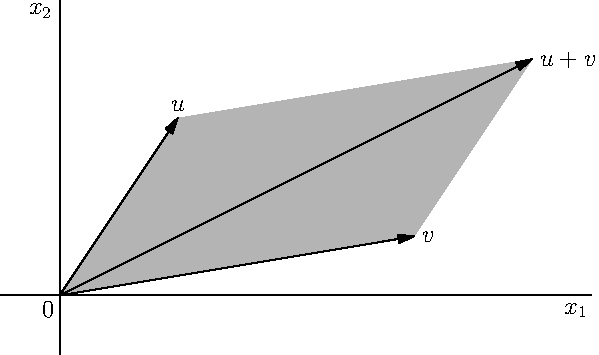
\includegraphics{vector_addition.pdf}
\end{center}
\end{law}\vspace{3ex}

所有元素都是零的向量称为\textbf{零向量}, 用\textbf{0}表示(\textbf{0}中元素的个数可由上下文确定)\\[2ex]

\begin{law}[$\mathbb{R}^n$中向量的代数性质]\ \\
对$\mathbb{R}^n$中一切向量$\mathbf{u}$,$\mathbf{v}$,$\mathbf{w}$以及标量$c$和$d$:
\begin{equation*}
\begin{array}{l@{}c@{}l l l@{}c@{}l l}
( & i & ) & \mathbf{u}+\mathbf{v}=\mathbf{v}+\mathbf{u} & ( & v & ) & c(\mathbf{u}+\mathbf{v})=c\mathbf{u}+c\mathbf{v}\\
( & ii & ) & (\mathbf{u}+\mathbf{v})+\mathbf{w}=\mathbf{u}+(\mathbf{v}+\mathbf{w}) & ( & vi & ) & (c+d)\mathbf{u}=c\mathbf{u}+d\mathbf{u}\\
( & iii & ) & \mathbf{u}+\mathbf{0}=\mathbf{0}+\mathbf{u}=\mathbf{u} & ( & vii & ) & c(d\mathbf{u})=(cd)\mathbf{u}\\
( & iv & ) & \mathbf{u}+(-\mathbf{u})=-\mathbf{u}+\mathbf{u}=\mathbf{0} & ( & viii & ) & 1\mathbf{u}=\mathbf{u}
\end{array}
\end{equation*}
\end{law}\vspace{2ex}

给定$\mathbb{R}^n$中向量$\mathbf{v}_1$,$\mathbf{v}_2$,$\cdots$,$\mathbf{v}_p$和标量$c_1$,$c_2$,$\cdots$,$c_p$, 向量
	\[\mathbf{y}=c_1\mathbf{v}_1+\cdots+c_p\mathbf{v}_p\]
称为向量$\mathbf{v}_1$,$\mathbf{v}_2$,$\cdots$,$\mathbf{v}_p$以$c_1$,$c_2$,$\cdots$,$c_p$为\textbf{权}的\textbf{线性组合}.\\[2ex]

\framebox{
\begin{minipage}{\linewidth}
向量方程
\[x_1\mathbf{a}_1+x_2\mathbf{a}_2+\cdots+x_n\mathbf{a}_n=\mathbf{b}\]
和增广矩阵为
\begin{equation}
[\mathbf{a}_1\quad\mathbf{a}_2\quad\cdots\quad\mathbf{a}_n\quad\mathbf{b}]\label{matrix:eq_01}
\end{equation}
的线性方程组有相同的解集. 特别地, $\mathbf{b}$可表示为$\mathbf{a}_1$,$\mathbf{a}_2$,$\cdots$,$\mathbf{a}_n$的线性组合当且仅当对应于\eqref{matrix:eq_01}式的线性方程组有解.
\end{minipage}}\\[4ex]

\begin{definition}
若$\mathbf{v}_1$,$\mathbf{v}_2$,$\cdots$,$\mathbf{v}_p$是$\mathbb{R}^n$中的向量, 则$\mathbf{v}_1$,$\mathbf{v}_2$,$\cdots$,$\mathbf{v}_p$的所有线性组合所成的组合用记号$\Span\{\mathbf{v}_1$,$\mathbf{v}_2$,$\cdots$,$\mathbf{v}_p\}$表示, 称为由$\mathbf{v}_1$,$\mathbf{v}_2$,$\cdots$,$\mathbf{v}_p$所\textbf{生成}(或\textbf{张成})\textbf{的$\mathbb{R}^n$的子集}. 也就是说, $\Span\{\mathbf{v}_1$,$\mathbf{v}_2$,$\cdots$,$\mathbf{v}_p\}$是所有形如
	\[c_1\mathbf{v}_1+c_2\mathbf{v}_2+\cdots+c_p\mathbf{v}_p\]
的向量的集合, 其中$c_1$,$c_2$,$\cdots$,$c_p$为标量.\\[2ex]
\end{definition}\vspace{4ex}

\section{矩阵方程$A\mathbf{x}=\mathbf{b}$}
\begin{definition}
若$A$是$m\times n$矩阵, 它的各列为$\bm{a}_1$,$\cdots$,$\bm{a}_n$. 若$\bm{x}$是$\mathbb{R}^n$中的向量, 则\textbf{$A$与$\bm{x}$的积}(记为$A\bm{x}$)就是\textbf{$A$的各列以$\bm{x}$中对应元素为权的线性组合}, 即
	\[A\bm{x}=[\bm{a}_1\ \bm{a}_2\ \cdots\ \bm{a}_n]\left[\begin{array}{c}x_1\\x_2\\\vdots\\x_n\end{array}\right]=x_1\bm{a}_1+x_2\bm{a}_2+\cdots+x_n\bm{a}_n\]
注意$A\bm{x}$仅当$A$的列数等于$\bm{x}$中的元素个数时才有意义.\\[2ex]
\end{definition}

\begin{TheoremOne}
若$A$是$m\times n$矩阵, 它的各列为$\bm{a}_1$,$\cdots$,$\bm{a}_n$, 而$\bm{b}$属于$\mathbb{R}^n$, 则矩阵方程
\[A\bm{x}=\bm{b}\]
与向量方程
\[x_1\bm{a}_1+x_2\bm{a}_2+\cdots+x_n\bm{a}_n=\bm{b}\]
有相同的解集. 它又与增广矩阵为
\[[\bm{a}_1\ \bm{a}_2\ \cdots\ \bm{a}_n\ \bm{b}]\]
的线性方程组有相同的解集.\\[2ex]
\end{TheoremOne}

\begin{center}
\framebox{
方程$Ax=b$有解当且仅当$b$是$A$的各列的线性组合
}
\end{center}\vspace{4ex}

\begin{TheoremOne}
设$A$是$m\times n$矩阵, 则下列命题是逻辑上等价的. 也就是说, 对某个$A$, 它们都成立或者都不成立.\\
\begin{tabular}{l@{\,}l}
a. & 对$\mathbb{R}^m$中每个$\bm{b}$, 方程$A\bm{x}=\bm{b}$有解.\\
b. & $\mathbb{R}^m$中的每个$\bm{b}$都是$A$的列的一个线性组合.\\
c. & $A$的各列生成$\mathbb{R}^m$.\\
d. & $A$在每一行都有一个主元位置.\\[2ex]
\end{tabular}
\end{TheoremOne}\vspace{2ex}

\begin{law}[计算$A\bm{x}$的行---向量规则]\ \\
若乘积$A\bm{x}$有定义, 则$A\bm{x}$中的第$i$个元素是$A$的第$i$行元素与$\bm{x}$的相应元素乘积之和.
\end{law}\vspace{2ex}

例1.\\
$\displaystyle a.\left[\begin{array}{r r r}
	1 & 2 & -1\\
	0 & -5 & 3
    \end{array}\right]
    \left[\begin{array}{r}
        4\\
	3\\
	7
    \end{array}\right]=
    \left[\begin{array}{r}
        1\cdot4+2\cdot3+(-1)\cdot7\\
	0\cdot4+(-5)\cdot3+3\cdot7
    \end{array}\right]=
    \left[\begin{array}{r}
        3\\
	6
    \end{array}\right]$\\[2ex]

$\displaystyle b.\left[\begin{array}{r r r}
	1 & 0 & 0\\
	0 & 1 & 0\\
	0 & 0 & 1
    \end{array}\right]
    \left[\begin{array}{r}
        r\\
	s\\
	t
    \end{array}\right]=
    \left[\begin{array}{r}
        1\cdot r+0\cdot s+0\cdot t\\
	0\cdot r+1\cdot s+0\cdot t\\
	0\cdot r+0\cdot s+1\cdot t
    \end{array}\right]=
    \left[\begin{array}{r}
	r\\
	s\\
	t
    \end{array}\right]$\\[2ex]

矩阵的主对角线上元素为1, 其他位置上元素为0, 这个矩阵称为\textbf{单位矩阵}, 并记为$I$.\\
如果矩阵为$n\times n$单位矩阵, 记为$I_n$.\\[2ex]

\begin{TheoremOne}
若$A$是$m\times n$矩阵, $\bm{u}$和$\bm{v}$是$\mathbb{R}^n$中向量, c是标量, 则\\
\begin{tabular}{l@{\,}l}
a. & $A(\bm{u}+\bm{v})=A\bm{u}+A\bm{v}$\\
b. & $A(c\bm{u})=c(A\bm{u})$
\end{tabular}
\end{TheoremOne}\vspace{6ex}

\section{线性方程组的解集}
若线性方程组可写成
\[A\bm{x}=\bm{0}\]
的形式, 则称为\textbf{齐次线性方程组}. 其中, $A$是$m\times n$矩阵, $\bm{0}$是$\mathbb{R}^m$中的零向量.\\
齐次线性方程组至少有一个解, 即$\bm{x}=\bm{0}$($\mathbb{R}^n$中的零向量), 这个解称为它的\textbf{平凡解}.\\
如果有一个非零向量$\bm{x}$, 满足$A\bm{x}=\bm{0}$, 这个解称为它的\textbf{非平凡解}.\\[2ex]

\begin{law}
齐次方程$A\bm{x}=\bm{0}$有非平凡解当且仅当方程至少有一个自由变量.
\end{law}\vspace{2ex}

$\bm{x}=s\bm{u}+t\bm{v}$为$A\bm{x}=\bm{0}$的\textbf{参数向量形式}, 并称之为\textbf{参数向量方程}. 其中, $s$,$t$为自由变量\\
$\bm{x}=\bm{p}+t\bm{v}$为$A\bm{x}=\bm{b}$的\textbf{参数向量形式}, 并称之为\textbf{参数向量方程}. 其中, $t$为自由变量\\[1ex]

例.\\
$x_1=0.3x_2+0.2x_3$\\[1ex]
$\bm{x}=
\left[\begin{array}{l}
x_1\\
x_2\\
x_3
\end{array}\right]=
\left[\begin{array}{c}
0.3x_2+0.2x_3\\
x_2\\
x_3
\end{array}\right]=
\left[\begin{array}{r}
0.3x_2\\
x_2\\
0
\end{array}\right]+\left[\begin{array}{r}
0.2x_3\\
0\\
x_3
\end{array}\right]\\
\phantom{\bm{x}}=x_2\left[\begin{array}{r}
0.3\\
1\\
0
\end{array}\right]+x_3\left[\begin{array}{r}
0.2\\
0\\
1
\end{array}\right]
$\\[2ex]
因此, $A\bm{x}=\bm{b}$的解集是一条通过$\bm{p}$而平行于$A\bm{x}=\bm{0}$的解集的直线. 也称为将$\bm{v}$沿着$\bm{p}$进行直线移动.\\[2ex]

\begin{TheoremOne}
设方程$A\bm{x}=\bm{b}$对某个$\bm{b}$是相容的, $\bm{p}$为一个特解, 则$A\bm{x}=\bm{b}$的解集是所有形如$\bm{w}=\bm{p}+\bm{v}_h$的向量的集, 其中$\bm{v}_h$时齐次方程$A\bm{x}=\bm{b}$的任意一个解.
\end{TheoremOne}\vspace{3ex}

\begin{law}[把(相容方程组的)解集表示成参数向量形式]\ \\
1.把增广矩阵简化为简化阶梯形.\\
2.把每个基本变量用自由变量表示.\\
3.把一般解$\bm{x}$表示成向量, 如果有自由变量, 其元素依赖于自由变量.\\
4.把$\bm{x}$分解为向量(元素为常数)的线性组合, 用自由变量作为参数.
\end{law}\vspace{4ex}

\section{线性方程组的应用}
1.经济学 - 部分的收支平衡\\[1ex]
例1.\\
假设一个经济体系由煤炭、电力和钢铁三个部门组成, 各部门之间的分配如下所示, 其中每一列中的数表示该部门总产出所占的比例. 设$p_C$,$p_E$,$p_S$分别为煤炭、电力和钢铁部门年度总产出的价格, 求出使每个部门收支平衡的产值.
\begin{table}[H]
\begin{tabular}{>{\centering\arraybackslash}p{0.2\textwidth}|>{\centering\arraybackslash}p{0.2\textwidth}|>{\centering\arraybackslash}p{0.2\textwidth}|>{\centering\arraybackslash}p{0.25\textwidth}}
    \hline
    \multicolumn{3}{c|}{\ziju{0.2}部门的产出分配} & \multirow{2}*{\ziju{0.8}采购部门}\\\cline{1-3}
    \ziju{1.5}煤炭 & \ziju{1.5}电力  & \ziju{1.5}钢铁 & \\\hline
    0.0 & 0.4 & 0.6 & 煤炭\\\hline
    0.6 & 0.1 & 0.2 & 电力\\\hline
    0.4 & 0.5 & 0.2 & 钢铁\\\hline
\end{tabular}
\caption{一个简单的经济问题}
\end{table}
解:\\
\[
    \left\{\begin{array}{r@{\hspace{2pt}}r@{\hspace{2pt}}r@{\hspace{2pt}}r@{\hspace{2pt}}r@{\hspace{2pt}}r@{\hspace{2pt}}r}
	p_C    & - & 0.4p_E & - & 0.6p_S & = & 0\\
	0.6p_C & - & 0.9p_E & + & 0.2p_S & = & 0\\
	0.4p_C & + & 0.5p_E & - & 0.8p_S & = & 0
    \end{array}\right.
\]
增广矩阵为:\\
$\displaystyle\left[\begin{array}{r r r r}
    5 & -2 & -3 & 0\\
    6 & -9 & 2 & 0\\
    4 & 5 & -8 & 0
\end{array}\right]$\\[1ex]

化简矩阵步骤:\\
1.5\ding{173}-6\ding{172}, 得:\\
$\displaystyle\left[\begin{array}{r r r r}
    5 & -2 & -3 & 0\\
    0 & -33 & 28 & 0\\
    4 & 5 & -8 & 0
\end{array}\right]$\\

2.5\ding{174}-4\ding{172}, 得:\\
$\displaystyle\left[\begin{array}{r r r r}
    5 & -2 & -3 & 0\\
    0 & -33 & 28 & 0\\
    0 & 33 & -28 & 0
\end{array}\right]$\\

3.\ding{174}+\ding{173}, 得:\\
$\displaystyle\left[\begin{array}{r r r r}
    5 & -2 & -3 & 0\\
    0 & -33 & 28 & 0\\
    0 & 0 & 0 & 0
\end{array}\right]$\\

4.33\ding{172}-2\ding{173}, 得:\\
$\displaystyle\left[\begin{array}{r r r r}
    165 & 0 & -155 & 0\\
    0 & -33 & 28 & 0\\
    0 & 0 & 0 & 0
\end{array}\right]$\\

5.化简主元, 得:\\
$\displaystyle\left[\begin{array}{r r r r}
    1 & 0 & -0.94 & 0\\
    0 & 1 & -0.85 & 0\\
    0 & 0 & 0 & 0
\end{array}\right]$\\[2ex]

2.化学式 - 等号两边原子守恒\\[2ex]

3.网络流 - 节点的进/出流量恒等\\
例2. 如下图, 该网络是巴尔的摩市区一些单行道在一个下午早些时候(以每小时车辆数目计算)的交通流量. 计算该网络的车流量\\
\begin{figure}[H]
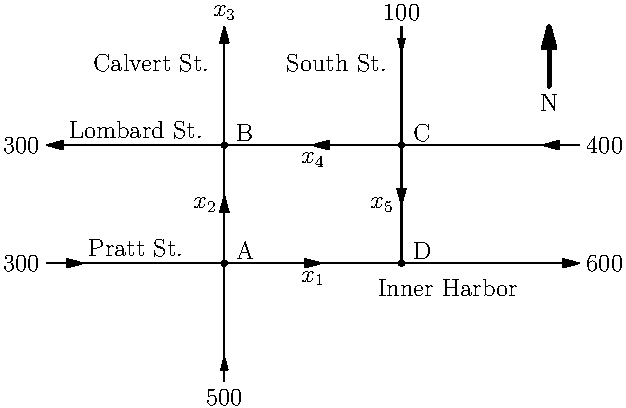
\includegraphics{traffic}
\caption{巴尔的摩道路}
\end{figure}
由每个路口的流量与总流量, 可得到方程组:
\[
\left\{\begin{array}{r r r r r r r r r r r}
    x_1 & + & x_2 & & & & & & & = & 800\\
    & & x_2 & - & x_3 & + & x_4 & & & = & 300\\
    & & & & x_3 & & & & & = & 400\\
    & & & & & & x_4 & + & x_5 & = & 500\\
    x_1 & & & & & & & + & x_5 & = & 600
\end{array}\right.
\]
对应的增广矩阵:
\[
\left[\begin{array}{r r r r r r}
    1 & 1 & 0 & 0 & 0 & 800\\
    0 & 1 & -1 & 1 & 0 & 300\\
    0 & 0 & 1 & 0 & 0 & 400\\
    0 & 0 & 0 & 1 & 1 & 500\\
    1 & 0 & 0 & 0 & 1 & 600
\end{array}\right]
\]
化简后的结果:
\[
\left[\begin{array}{r r r r r r}
    1 & 0 & 0 & 0 & 1 & 600\\
    0 & 1 & 0 & 0 & -1 & 200\\
    0 & 0 & 1 & 0 & 0 & 400\\
    0 & 0 & 0 & 1 & 1 & 500
\end{array}\right]
\]
所以
\[
x=\left\{\begin{array}{c}
    x_1\\
    x_2\\
    x_3\\
    x_4\\
    x_5
\end{array}\right.=\left[\begin{array}{r@{\hspace{1pt}}r@{\hspace{1pt}}r}
    600 & - & x_5\\
    200 & + & x_5\\
    400 & &\\
    500 & - & x_5\\
    & & x_5
\end{array}\right]=\left[\begin{array}{r}
    600\\
    200\\
    400\\
    500\\
    0
\end{array}\right]+\left[\begin{array}{r}
    -1\\
    1\\
    0\\
    -1\\
    1
\end{array}\right]x_5
\]\\[4ex]

\section{线性无关}
\begin{definition}
$\mathbb{R}^n$中一组向量$\{\bm{v}_1$,$\cdots$,$\bm{v}_p\}$称为\textbf{线性无关}的, 若向量方程
\[x_1\bm{v}_1+x_2\bm{v}_2+\cdots+x_p\bm{v}_p=\bm{0}\]
仅有平凡解. 向量组(集)$\{\bm{v}_1$,$\cdots$,$\bm{v}_p\}$称为\textbf{线性相关}的, 若存在不全为零的权$c_1$,$\cdots$,$c_p$, 使
\[c_1\bm{v}_1+c_2\bm{v}_2+\cdots+c_p\bm{v}_p=\bm{0}\]
\end{definition}\vspace{2ex}

\begin{law}
矩阵$A$的各列线性无关, 当且仅当方程$A\bm{x}=\bm{0}$仅有平凡解.
\end{law}\vspace{2ex}

例1.\\
确定矩阵$\displaystyle A=\left[\begin{array}{r r r}
    0 & 1 & 4\\
    1 & 2 & -1\\
    5 & 8 & 0
\end{array}\right]$的各列是否线性无关\\
解.\\
将增广矩阵进行化简:\\
\[
\left[\begin{array}{r r r r}
    0 & 1 & 4 & 0\\
    1 & 2 & -1 & 0\\
    5 & 8 & 0 & 0
\end{array}\right]\sim\left[\begin{array}{r r r r}
    1 & 2 & -1 & 0\\
    0 & 1 & 4 & 0\\
    0 & -2 & 5 & 0
\end{array}\right]\sim\left[\begin{array}{r r r r}
    1 & 2 & -1 & 0\\
    0 & 1 & 4 & 0\\
    0 & 0 & 13 & 0
\end{array}\right]
\]
由于方程没有自由变量, 因此方程$A\bm{x}=\bm{0}$只有平凡解.\\[2ex]

\begin{law}
两个向量的集合$\{\bm{v}_1$,$\bm{v}_2\}$线性相关, 当且仅当其中一个向量是另一个向量的倍数. 这个集合线性无关, 当且仅当其中任一个向量都不是另一个向量的倍数.
\end{law}\vspace{4ex}

\begin{TheoremTwo}[线性相关集的特征]
两个或更多个向量的集合$S=\{\bm{v}_1,\cdots,\bm{v}_p\}$线性相关, 当且仅当S中至少有一个向量是其他向量的线性组合. 事实上, 若S线性相关, 且$\bm{v}_1\neq\bm{0}$, 则某个$\bm{v}_j$$(j>1)$是它前面向量$\bm{v}_1$,$\cdots$,$\bm{v}_{j-1}$的线性组合.
\end{TheoremTwo}\vspace{4ex}

\begin{TheoremOne}
若一个向量组的向量个数超过每个向量的元素个数, 那么这个向量组线性相关. 就是说, $\mathbb{R}^n$中任意向量组$\{\bm{v}_1$,$\cdots$,$\bm{v}_p\}$当$p>n$时线性相关.
\end{TheoremOne}\vspace{4ex}

\begin{TheoremOne}
若$\mathbb{R}^n$中向量组$S=\{\bm{v}_1,\cdots,\bm{v}_p\}$包含零向量, 则它线性相关.
\end{TheoremOne}\vspace{4ex}

\section{线性变换介绍}
由$\bm{x}$到$A\bm{x}$的对应是由一个向量集到另一个向量集的函数\\[2ex]

\begin{definition}
变换(或映射)$T$称为\textbf{线性}的, 若\\
\begin{tabular}{l@{}c@{}l@{\hspace{2pt}}l}
$($ & i & $)$ & 对$T$的定义域中一切$\bm{u}$,$\bm{v}$,$T(\bm{u}+\bm{v})=T(\bm{u})+T(\bm{v})$.\\
$($ & ii & $)$ & 对$T$的定义域中的一切$\bm{u}$和数$c$, $T(c\bm{u})=cT(\bm{u})$.
\end{tabular}
\end{definition}\vspace{4ex}

\begin{law}
若T是线性变换, 则
\[T(\bm{0})=\bm{0}\]
且对$T$的定义域中一切向量$\bm{u}$和$\bm{v}$以及数$c$和$d$, 有:
\[T(c\bm{u}+d\bm{v})=cT(\bm{u})+dT(\bm{v})\]
\end{law}\vspace{2ex}

给定数$r$, 定义$T:\mathbb{R}^2\rightarrow\mathbb{R}^2$为$T(\bm{x})=r\bm{x}$. 当$0\leqslant r\leqslant 1$时, $T$称为\textbf{压缩变换}; 当$r>1$时, $T$称为\textbf{拉伸变换}.\\[4ex]

\section{线性变换的矩阵}
\begin{TheoremOne}
设$T$:$\mathbb{R}^n\rightarrow\mathbb{R}^m$为线性变换, 则存在唯一的矩阵$A$, 使得对$\mathbb{R}^n$中一切$\bm{x}$, 有
\[T(\bm{x})=A\bm{x}\]
事实上, $A$是$m\times n$矩阵, 它的第$j$列是向量$T(\bm{e}_j)$, 其中$\bm{e}_j$是$\mathbb{R}^n$中单位矩阵$\bm{I}_n$的第$j$列:
\[A=[T(\bm{e}_1)\ \cdots\ T(\bm{e}_n)]\]
\end{TheoremOne}\vspace{4ex}

\begin{definition}
映射$T$:$\mathbb{R}^n\rightarrow\mathbb{R}^m$称为到$\mathbb{R}^m$上的映射, 若$\mathbb{R}^m$中每个$\bm{b}$是$\mathbb{R}^n$中至少一个$\bm{x}$的像(也称为\textbf{满射}).
\end{definition}\vspace{4ex}

\begin{definition}
映射$T$:$\mathbb{R}^n\rightarrow\mathbb{R}^m$称为\textbf{一对一映射}(或1:1), 若$\mathbb{R}^m$中每个$\bm{b}$是$\mathbb{R}^n$中至多一个$\bm{x}$的像(也称为\text{单射}).
\end{definition}\vspace{4ex}

\begin{TheoremOne}
设$T$:$\mathbb{R}^n\rightarrow\mathbb{R}^m$为线性变换, 则$T$是一对一的当且仅当方程$A\bm{x}=\bm{0}$仅有平凡解.
\end{TheoremOne}\vspace{4ex}

\begin{TheoremOne}
设$T$:$\mathbb{R}^n\rightarrow\mathbb{R}^m$是线性变换, 设$A$为$T$的标准矩阵, 则\\
\begin{tabular}{l@{\ }l}
a. & $T$把$\mathbb{R}^n$映上到$\mathbb{R}^m$, 当且仅当$A$的列生成$\mathbb{R}^m$.\\
b. & $T$是一对一的, 当且仅当$A$的列线性无关.
\end{tabular}
\end{TheoremOne}\vspace{2ex}

\begin{longtable}{>{\raggedright}m{0.35\linewidth}>{\centering}m{0.35\linewidth}>{\centering\arraybackslash}m{0.25\linewidth}}
\hline
变换名称 & 变换图像 & 标准矩阵\\\hline
旋转 & \raisebox{0pt}[4.2cm][0.2cm]{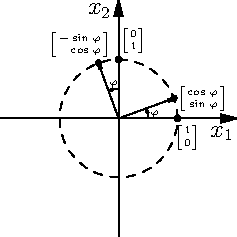
\includegraphics[totalheight=4cm]{rotate}} & $\left[\begin{array}{r r}\cos\varphi & -\sin\varphi\\ \sin\varphi & \cos\varphi\end{array}\right]$\\\hline
关于$x$轴对称 & \raisebox{0pt}[4.2cm][0.2cm]{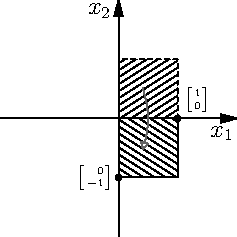
\includegraphics[totalheight=4cm]{symmetry_01}} & $\left[\begin{array}{r r} 1 & 0\\ 0 & -1\end{array}\right]$\\\hline
关于$y$轴对称 & \raisebox{0pt}[4.2cm][0.2cm]{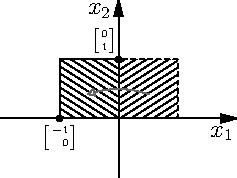
\includegraphics[totalheight=4cm]{symmetry_02}} & $\left[\begin{array}{r r} -1 & 0\\ 0 & 1\end{array}\right]$\\\hline
关于直线$y=x$对称 & \raisebox{0pt}[4.2cm][0.2cm]{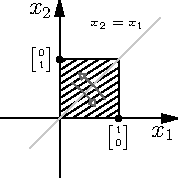
\includegraphics[totalheight=4cm]{symmetry_03}} & $\left[\begin{array}{r r} 0 & 1\\ 1 & 0\end{array}\right]$\\\hline
关于直线$y=-x$对称 & \raisebox{0pt}[4.2cm][0.2cm]{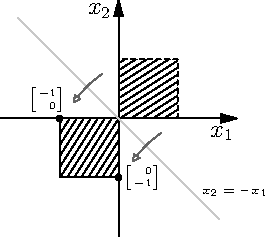
\includegraphics[totalheight=4cm]{symmetry_04}} & $\left[\begin{array}{r r} 0 & -1\\ -1 & 0\end{array}\right]$\\\hline
关于原点对称 & \raisebox{0pt}[4.2cm][0.2cm]{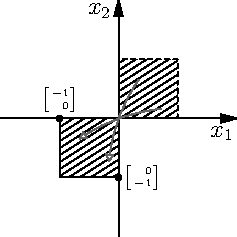
\includegraphics[totalheight=4cm]{symmetry_05}} & $\left[\begin{array}{r r} -1 & 0\\ 0 & -1\end{array}\right]$\\\hline
沿$x$轴拉伸 & \raisebox{0pt}[4.2cm][0.2cm]{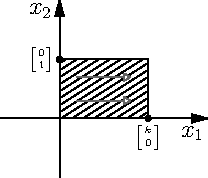
\includegraphics[totalheight=4cm]{scale_01}} & $\left[\begin{array}{r r} k & 0\\ 0 & 1\end{array}\right]$\\\hline
沿$y$轴拉伸 & \raisebox{0pt}[4.2cm][0.2cm]{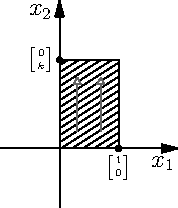
\includegraphics[totalheight=4cm]{scale_02}} & $\left[\begin{array}{r r} 1 & 0\\ 0 & k\end{array}\right]$\\\hline
沿$x$轴倾斜 & \raisebox{0pt}[4.2cm][0.2cm]{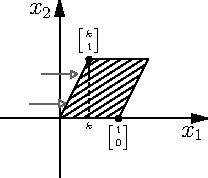
\includegraphics[totalheight=4cm]{slant_01}} & $\left[\begin{array}{r r} 1 & k\\ 0 & 1\end{array}\right]$\\\hline
沿$y$轴倾斜 & \raisebox{0pt}[4.2cm][0.2cm]{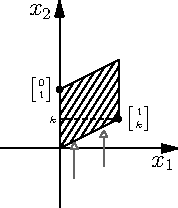
\includegraphics[totalheight=4cm]{slant_02}} & $\left[\begin{array}{r r} 1 & 0\\ k & 1\end{array}\right]$\\\hline
投影到$x$轴 & \raisebox{0pt}[4.2cm][0.2cm]{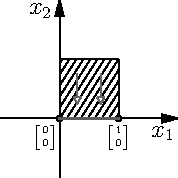
\includegraphics[totalheight=4cm]{shadow_01}} & $\left[\begin{array}{r r} 1 & 0\\ 0 & 0\end{array}\right]$\\\hline
投影到$y$轴 & \raisebox{0pt}[4.2cm][0.2cm]{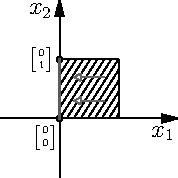
\includegraphics[totalheight=4cm]{shadow_02}} & $\left[\begin{array}{r r} 0 & 0\\ 0 & 1\end{array}\right]$\\\hline
\caption{线性变换一览}
\end{longtable}\vspace{6ex}

\section{商业、科学和工程中的线性模型}
例1. 如表格所示, 代表食谱中的三种食物以及100克每种食物成分含有某些营养素的数量. 求出脱脂牛奶、大豆粉和乳清的某种组合, 使该食谱每天能供给如图表所需的蛋白质、碳水化合物和脂肪的含量.\\
\begin{table}[H]
\begin{tabular}{l c c c c}

\end{tabular}
\end{table}

\begin{law}[基尔霍夫电压定律]\ \\
围绕一条回路同一方向的电压降$RI$的代数和等于围绕该回路的同一方向电动势的代数和.
\end{law}\vspace{4ex}

\begin{law}
如果有矩阵$A$使$\bm{x}_1=A\bm{x}_0$,$\bm{x}_2=A\bm{x}_1$, 一般地,
\[\bm{x}_{k+1}=A\bm{x}_k\text{,\ }k=0,1,2,\cdots\]
则称为\textbf{线性差分方程}(或\textbf{递归关系}).
\end{law}

\documentclass[UTF8,fontset=ubuntu]{ctexart}
\usepackage{amsmath}
\usepackage{bm}
\usepackage{parskip}
\usepackage{amssymb}
\usepackage{xcolor}
\usepackage{colortbl}
\usepackage{framed}
\usepackage[framed]{ntheorem}
\theoremheaderfont{\normalfont\bfseries}
\theorembodyfont{\slshape}
\theoremseparator{\hspace{2ex}}
\theoremindent2ex
\theoremstyle{plain}
\newtheorem{theorem}{定理}
\theoremstyle{nonumberplain}
\newtheorem{definition}{定义}
\theoremstyle{empty}
\newframedtheorem{law}{定律}
\definecolor{lightgray}{gray}{0.7}
\definecolor{gray}{gray}{0.5}
\definecolor{white}{gray}{1}
\begin{document}
一、矩阵运算\\[1ex]
$m\times n$矩阵$A=[a_{ij}]$的\textbf{对角线元素}是$a_{11}$,$a_{22}$,$a_{33}$,$\cdots$, 它们组成$A$的\textbf{主对角线}.\\[1ex]
\textbf{对角矩阵}是一个方阵, 它的非对角线元素全是0. 例如$n\times n$单位矩阵$\bm{I}_n$.\\[1ex]
元素全是0的$m\times n$矩阵称为\textbf{零矩阵}, 用$\bm{0}$表示.\\[1ex]
若两个矩阵有相同的维数(即有相同的行数和列数), 而且对应元素相同, 则称该两个矩阵\textbf{相等}\\[1ex]
若$r$是标量而$A$是矩阵, 则\textbf{标量乘法}$rA$是一个矩阵, 它的每一列是$A$的对应列的$r$倍.\\[2ex]

\begin{theorem}
设$A$,$B$,$C$是相同维数的矩阵, $r$与$s$为数, 则有\\
\begin{tabular}{l@{\ }l@{\hspace{5em}}l@{\ }l}
a. & $A+B=B+A$ & b. & $(A+B)+C=A+(B+C)$\\
c. & $A+0=A$ & d. & $r(A+B)=rA+rB$\\
e. & $(r+s)A=rA+sA$ & f. & $r(sA)=(rs)A$
\end{tabular}
\end{theorem}\vspace{4ex}

\begin{definition}
若$A$是$m\times n$矩阵, $B$是$n\times p$矩阵, $B$的列是$\bm{b}_1$,$\cdots$,$\bm{b}_p$, 则乘积$AB$是$m\times p$矩阵, 它的各列是$A\bm{b}_1$,$\cdots$,$A\bm{b}_p$, 即
\[AB=A[\bm{b}_1\ \bm{b}_2\ \cdots\ \bm{b}_p]=[A\bm{b}_1\ A\bm{b}_2\ \cdots\ A\bm{b}_p]\]
\end{definition}\vspace{4ex}

\begin{law}
$AB$的每一列都是$A$的各列的线性组合, 以$B$的对应列的元素为权.
\end{law}\vspace{4ex}

\begin{law}[计算$AB$的行列法则]\ \\
若乘积$AB$有定义, 则$AB$的第$i$行第$j$列的元素是$A$的第$i$行与$B$的第$j$列对应元素乘积之和. 若($AB$)${}_{ij}$表示$AB$的($i$,$j$)元素, $A$为$m\times n$矩阵, 则
\[(AB)_{ij}=a_{i1}b_{1j}+a_{i2}b_{2j}+\cdots+a_{in}b_{nj}\]
\end{law}\vspace{4ex}

\begin{theorem}
设$A$为$m\times n$矩阵, $B$和$C$的维数使下列各式的乘积有意义.\\
\begin{tabular}{l@{\ }l l}
a. & $A(BC)=(AB)C$ & (乘法结合律)\\
b. & $A(B+C)=AB+AC$ & (乘法左分配律)\\
c. & $(B+C)A=BA+CA$ & (乘法右分配律)\\
d. & $r(AB)=(rA)B=A(rB)$, r为任意数 &\\
e. & $I_mA=A=AI_m$ & (矩阵乘法的恒等式)
\end{tabular}
\end{theorem}\vspace{4ex}

乘积$AB$的因子关系为: $A$被$B$\textbf{右乘}, 或$B$被$A$\textbf{左乘}\\
若$AB$=$BA$, 我们称$A$和$B$彼此\textbf{可交换}\\[2ex]

\textbf{警告}\\
1.一般情况下, $AB\neq BA$.\\
2.消去律对矩阵乘法不成立, 即若$AB=AC$, 一般情况下, $B=C$并不成立.\\
3.若乘积$AB$是零矩阵, 一般情况下, 不能断定A=0或B=0.\\[2ex]

给定$m\times n$矩阵, 则$A$的\textbf{转置}是一个$n\times m$矩阵, 用$A^T$表示, 它的列是由$A$的对应行构成的.\\[2ex]

\begin{theorem}
设$A$与$B$表示矩阵, 其维数使下列和与积有定义, 则\\
\begin{tabular}{l@{\ }l}
a. & $(A^T)^T=A$.\\
b. & $(A+B)^T=A^T+B^T$.\\
c. & 对任意数$r$, $(rA)^T=rA^T$.\\
d. & $(AB)^T=B^TA^T$.
\end{tabular}
\end{theorem}\vspace{4ex}

\begin{law}
若干个矩阵的乘积的转置等于它们的转置的乘积, 但相乘的顺序相反.
\end{law}\vspace{8ex}

二、矩阵的逆\\[1ex]
$A$为$n\times n$矩阵, 若存在一个$n\times n$矩阵$C$, 使得
\[CA=\bm{I}_n\qquad\text{且}AC=\bm{I}_n\]
则称$A$\textbf{可逆}, 并且$C$是$A$的\textbf{逆}.\\[2ex]
若$A$可逆, 它的逆是唯一的, 我们将它记为$A^{-1}$, 则
\[A^{-1}A=I\qquad\text{且}AA^{-1}=I\]
不可逆矩阵也称为\textbf{奇异矩阵}.\\
可逆矩阵也称为\textbf{非奇异矩阵}.\\[2ex]

\begin{theorem}
设$A=\left[\begin{array}{r r}3 & 4\\5 & 6\end{array}\right]$. 若$ad-bc\neq 0$, 则$A$可逆且
\[A^{-1}=\frac{1}{ad-bc}\left[\begin{array}{l l}d & -b\\-c & a\end{array}\right]\]
若$ad-bc=0$, 则$A$不可逆.
\end{theorem}\vspace{4ex}

数$ad-bc$称为$A$的\textbf{行列式}, 记为
\[\det A=ad-bc\]\\

\begin{theorem}
若$A$是可逆$n\times n$矩阵, 则对每一$\mathbb{R}^n$中的$\bm{b}$, 方程$A\bm{x}=\bm{b}$有唯一解$\bm{x}=A^{-1}\bm{b}$.
\end{theorem}\vspace{4ex}

\begin{law}[胡克定律]\ \\
公式如下
\[\bm{y}=D\bm{f}\]
其中$D$为\textbf{弹性矩阵}, 它的逆称为\textbf{刚性矩阵}, $\bm{f}$表示它在各个点受的力, $\bm{y}$表示各个点的形变量.
\end{law}\vspace{4ex}

\begin{theorem}\ \\
a.若$A$是可逆矩阵, 则$A^{-1}$也可逆而且$(A^{-1})^{-1}=A$.\\
b.若$A$和$B$都是$n\times n$可逆矩阵, 则$AB$也可逆, 且其逆是$A$和$B$的逆矩阵按相反顺序的乘积, 即
\[(AB)^{-1}=B^{-1}A^{-1}\]
c.若$A$可逆, 则$A^T$也可逆, 且其逆是$A^{-1}$的转置, 即$(A^T)^{-1}=(A^{-1})^T$.
\end{theorem}\vspace{4ex}

\begin{law}
若干个$n\times n$可逆矩阵的积也是可逆的, 其逆等于这些矩阵的逆按相反顺序的乘积.
\end{law}\vspace{4ex}

把单位矩阵进行一次初等行变换, 就得到\textbf{初等矩阵}.\\[2ex]

\begin{law}
若对$m\times n$矩阵$A$进行某种初等行变换, 所得矩阵可写成$EA$, 其中$E$是$m\times m$矩阵, 是由$I_m$进行同一行变换所得.
\end{law}\vspace{4ex}

\begin{law}
每个初等矩阵$E$是可逆的, $E$的逆是一个同类型的初等矩阵, 它把$E$变回$I$.
\end{law}\vspace{4ex}

\begin{theorem}
$n\times n$矩阵$A$是可逆的, 当且仅当$A$行等价于$I_n$, 这时, 把$A$化简为$I_m$的一系列初等行变化同时把$I_n$变成$A^{-1}$.
\end{theorem}\vspace{4ex}

\begin{law}[求$A^{-1}$的算法]\ \\
把增广矩阵$[A\ I]$进行行化简. 若$A$行等价于$I$, 则$[A\ I]$行等价于$[I\ A^{-1}]$, 否则$A$没有逆.
\end{law}\vspace{8ex}

三、可逆矩阵的特征\\[-3ex]
\begin{theorem}[可逆矩阵定理]
设$A$为$n\times n$矩阵, 则下列命题是等价的, 即对某一特定的$A$, 它们同时为真或同时为假.\\
\begin{tabular}{l@{\ }l}
a. & $A$是可逆矩阵.\\
b. & $A$行等价于$n\times n$单位矩阵.\\
c. & $A$有$n$个主元位置.\\
d. & 方程$A\bm{x}=\bm{0}$仅有平凡解.\\
e. & $A$的各列线性无关.\\
f. & 线性变换$\bm{x}\mapsto A\bm{x}$是一对一的.\\
g. & 对$\mathbb{R}^n$中任意$\bm{b}$, 方程$A\bm{x}=\bm{b}$至少有一个解.\\
h. & $A$的各列生成$\mathbb{R}^n$,\\
i. & 线性变换$\bm{x}\mapsto A\bm{x}$把$\mathbb{R}^n$映上到$\mathbb{R}^n$.\\
j. & 存在$n\times n$矩阵$C$使$CA=I$.\\
k. & 存在$n\times n$矩阵$D$使$AD=I$.\\
l. & $A^T$是可逆矩阵.
\end{tabular}
\end{theorem}\vspace{4ex}

\begin{law}
设$A$和$B$为方阵, 若$AB=I$, 则$A$和$B$都是可逆的, 且$B=A^{-1}$, $A=B^{-1}$.
\end{law}\vspace{4ex}

\begin{theorem}
设$T$:$\mathbb{R}^n\rightarrow\mathbb{R}^n$为线性变换, $A$为$T$的标准矩阵. 则$T$可逆当且仅当$A$是可逆矩阵.
\end{theorem}\vspace{4ex}

若一个$m\times n$矩阵的主对角线以下元素全为0, 则称之为\textbf{上三角矩阵}.\\[1ex]
若一个$m\times n$矩阵的主对角线以上元素全为0, 则称之为\textbf{下三角矩阵}.\\[4ex]

四、分块矩阵\\[1ex]
形如
\[A=\left[
\begin{array}{r r r|r r|r}
3 & 0 & -1 & 5 & 9 & -2\\
-5 & 2 & 4 & 0 & -3 & 1\\\hline
-8 & -6 & 3 & 1 & 7 & -4
\end{array}
\right]\]
为矩阵$A$的$2\times 3$\textbf{分块矩阵}, 也可表示为
\[A=\left[
\begin{array}{l l l}
A_{11} & A_{12} & A_{13}\\
A_{21} & A_{22} & A_{23}
\end{array}
\right]\]\\[2ex]

设$A$为$m\times n$矩阵, $B$为$n\times p$矩阵, 当$A$的列的分法与$B$的行的分法一致时, 可计算$AB$. 如下:
\[A=\left[\begin{array}{r r r|r r}
2 & -3 & 1 & 0 & -4\\
1 & 5 & -2 & 3 & -1\\\hline
0 & -4 & -2 & 7 & -1
\end{array}\right]=
\left[\begin{array}{l l}
A_{11} & A_{12}\\
A_{21} & A_{22}
\end{array}\right]\]
\[B=\left[\begin{array}{r r}
6 & 4\\
-2 & 1\\
-3 & 7\\\hline
-1 & 3\\
5 & 2
\end{array}\right]=
\left[\begin{array}{l}
B_1\\
B_2
\end{array}\right]\]
\[AB=\left[
\begin{array}{l l}
A_{11} & A_{12}\\
A_{21} & A_{22}
\end{array}
\right]\left[
\begin{array}{l}
B_1\\
B_2
\end{array}
\right]=\left[
\begin{array}{l}
A_{11}B_1+A_{12}B_2\\
A_{21}B_1+A_{22}B_2
\end{array}
\right]=\left[
\begin{array}{r r}
-5 & 4\\
-6 & 2\\\hline
2 & 1
\end{array}
\right]\]\\[2ex]

\begin{theorem}[$AB$的列行展开]\ \\
若$A$是$m\times n$矩阵, $B$是$n\times p$矩阵, 则
\[\begin{array}{l@{}l}
AB & =[col_1(A)\ col_2(A)\ \cdots\ col_n(A)]\left[
\begin{array}{c}
row_1(B)\\
row_2(B)\\
\vdots\\
row_n(B)
\end{array}
\right]\\
& =col_1(A)row_1(B)+\cdots+col_n(A)row_n(B)
\end{array}\]
\end{theorem}\vspace{8ex}

五、矩阵因式分解\\[1ex]
设$A$是$m\times n$矩阵, 它可以行化简为阶梯形(化简步骤不包含对换变换), 则$A$可写成$A=LU$. 其中, $L$是$m\times m$下三角矩阵, 主对角线元素全是1; $U$是$A$的一个$m\times n$阶梯形矩阵.\\[2ex]

\begin{law}[$LU$分解的算法]\ \\
1.如果可能的话, 用一系列的行倍加变换把$A$化为阶梯形$U$(即$L^{-1}A=U$).\\
2.填充$L$的元素使相同的行变换把$L$变为$I$.
\end{law}\vspace{4ex}

$LU$分解图解:\\
\[\begin{array}{c@{}c@{}c@{}c@{}c@{}c@{}c@{}c@{}c}
A= & \left[\hspace{-1ex}\begin{array}{>{\columncolor{lightgray}[0pt]}r r r r}
\cellcolor{gray}2 & 4 & 5 & -2\\
-4 & -5 & -8 & 1\\
2 & -5 & 1 & 8\\
-6 & 0 & -3 & 1
\end{array}\hspace{-1ex}\right] & \Rightarrow & \left[\!\begin{array}{r >{\columncolor{white}[0pt]}r r r}
2 & 4 & 5 & -2\\
0 & \cellcolor{gray}3 & 2 & -3\\
0 & \cellcolor{lightgray}-9 & -4 & 10\\
0 & \cellcolor{lightgray}12 & 12 & -5
\end{array}\hspace{-1ex}\right] & \Rightarrow & \left[\!\begin{array}{r r >{\columncolor{white}[6pt][0pt]}r r}
2 & 4 & 5 & -2\\
0 & 3 & 2 & -3\\
0 & 0 & \cellcolor{gray}2 & 1\\
0 & 0 & \cellcolor{lightgray}4 & 7
\end{array}\hspace{-1ex}\right] & \Rightarrow & \left[\!\begin{array}{r r r >{\columncolor{white}[0pt]}r}
2 & 4 & 5 & -2\\
0 & 3 & 2 & -3\\
0 & 0 & 2 & 1\\
0 & 0 & 0 & \cellcolor{gray}5
\end{array}\hspace{-1ex}\right] & =U\\
& \downarrow & & \downarrow & & \downarrow & & \downarrow &\\
 & \left[\hspace{-1ex}\begin{array}{>{\columncolor{lightgray}[0pt]}r r r r}
\cellcolor{gray}1 & 0 & 0 & 0\\
-2 & 1 & 0 & 0\\
1 & & 1 & 0\\
-3 & & & 1
\end{array}\hspace{-1ex}\right] & & \left[\!\begin{array}{r >{\columncolor{white}[0pt]}r r r}
1 & 0 & 0 & 0\\
-2 & \cellcolor{gray}1 & 0 & 0\\
1 & \cellcolor{lightgray}-3 & 1 & 0\\
-3 & \cellcolor{lightgray}4 & & 1
\end{array}\hspace{-1ex}\right] & & \left[\!\begin{array}{r r >{\columncolor{white}[6pt][0pt]}r r}
1 & 0 & 0 & 0\\
-2 & 1 & 0 & 0\\
1 & -3 & \cellcolor{gray}1 & 0\\
-3 & 4 & \cellcolor{lightgray}2 & 1
\end{array}\hspace{-1ex}\right] & & \left[\!\begin{array}{r r r >{\columncolor{white}[6pt][0pt]}r}
1 & 0 & 0 & 0\\
-2 & 1 & 0 & 0\\
1 & -3 & 1 & 0\\
-3 & 4 & 2 & \cellcolor{gray}1
\end{array}\!\right] & =L
\end{array}\]\\[4ex]

六、列昂惕夫投入产出模型\\[-3ex]
\begin{law}[列昂惕夫投入产出模型或生产方程]\ \\
\[\bm{x}=C\bm{x}+\bm{d}\]
\end{law}\vspace{4ex}

\begin{theorem}
设$C$为某一经济体系的消耗矩阵, $\bm{d}$为最终需求. 若$C$和$\bm{d}$的元素非负, $C$的每一列的和小于1, 则$(I-C)^{-1}$存在, 产出向量
\[\bm{x}=(I-C)^{-1}\bm{d}\]
有非负元素, 且是下列方程的唯一解:
\[\bm{x}=C\bm{x}+d\]
\end{theorem}\vspace{8ex}

七、计算机图形学中的应用\\[1ex]
物体的平移并不直接对应于矩阵乘法, 因为平移并非线性变换, 所以引入\textbf{齐次坐标}\\[1ex]
$\mathbb{R}^2$中每个点$(x,y)$对应于$\mathbb{R}^3$中的点$(x,y,1)$, $(x,y,1)$为$(x,y)$的\textbf{齐次坐标}\\[1ex]
$(x,y,1)\mapsto(x+h,y+k,1)$的平移变换实现:\\
\[\left[\begin{array}{r r r}
1 & 0 & h\\
0 & 1 & k\\
0 & 0 & 1
\end{array}\right]
\left[\begin{array}{r}
x\\
y\\
1
\end{array}\right]=
\left[\begin{array}{c}
x+h\\
y+k\\
1
\end{array}\right]\]\\[2ex]
$\mathbb{R}^2$中任意线性变换可以通过齐次坐标乘以分块矩阵$\left[\begin{array}{r r}A & 0\\0 & 1\end{array}\right]$实现, 其中$A$是$2\times 2$矩阵.\\[2ex]
$(x,y,z,1)$是$\mathbb{R}^3$中点$(x,y,z)$的齐次坐标. 若$H\neq 0$, 则$(X,Y,Z,H)$为$(x,y,z)$的齐次坐标, 且
\[x=\frac{X}{H},y=\frac{Y}{H},z=\frac{Z}{H}\]\\[1ex]
点$(x,y,z)$在$xy$平面上的透视投影坐标为$(\dfrac{x}{1-z/d}, \dfrac{y}{1-z/d}, 0)$. 其中, $d$为$z$轴观测位置$(0,0,d)$\\[2ex]
绕$\mathbb{R}^2$中一点$p$的旋转是这样实现的: 首先把图形平移$-p$, 然后绕原点旋转, 最后平移$p$.
\end{document}

% \documentclass[UTF8, fontset=ubuntu]{ctexart}
% \usepackage{amsmath}
% \usepackage{amssymb}
% \usepackage{parskip}
% \usepackage{cancel}
% \usepackage{ntheorem}
% \theoremheaderfont{\normalfont\bfseries}
% \theorembodyfont{\slshape}
% \theoremseparator{\hspace{2ex}}
% \theoremindent2ex
% \theoremstyle{nonumberplain}
% \newtheorem{definition}{定义}
% \theoremstyle{plain}
% \newtheorem{theorem}{定理}
% \begin{document}
\part{行列式}
\section{一、行列式介绍}
有$3\times 3$矩阵$A$
\[\left[\begin{array}{l l l}
a_{11} & a_{12} & a_{13}\\
a_{21} & a_{22} & a_{23}\\
a_{31} & a_{32} & a_{33}
\end{array}\right]\]
其中
\[\Delta=a_{11}a_{22}a_{33}+a_{12}a_{23}a_{31}+a_{13}a_{21}a_{32}-a_{11}a_{23}a_{32}-a_{12}a_{21}a_{33}-a_{13}a_{22}a_{31}\]
$\Delta$称为$3\times 3$矩阵$A$的\textbf{行列式}, 也可以写成\\
$\Delta=(a_{11}a_{22}a_{33}-a_{11}a_{23}a_{32})-(a_{12}a_{21}a_{33}-a_{12}a_{23}a_{31})+(a_{13}a_{21}a_{32}-a_{13}a_{22}a_{31})$\\[1ex]
$\phantom{\Delta}=a_{11}\cdot\det\left[\begin{array}{l l}
a_{22} & a_{23}\\
a_{32} & a_{33}
\end{array}\right]-a_{12}\cdot\det\left[\begin{array}{l l}
a_{21} & a_{23}\\
a_{31} & a_{33}
\end{array}\right]+a_{13}\cdot\det\left[\begin{array}{l l}
a_{21} & a_{22}\\
a_{31} & a_{32}
\end{array}\right]$\\[1ex]
$\phantom{\Delta}=a_{11}\cdot\det A_{11}-a_{12}\cdot\det A_{12}+a_{13}\cdot\det A_{13}$\\
其中, $A_{ij}$表示去除矩阵第$i$行和第$j$列元素后的内容.\\
例. $A_{11}$表示如下:\\
\[\left[\begin{array}{l l l}
\cancel{a_{11}} & \cancel{a_{12}} & \cancel{a_{13}}\\
\cancel{a_{21}} & a_{22} & a_{23}\\
\cancel{a_{31}} & a_{32} & a_{33}
\end{array}\right]\]
即
\[\left[\begin{array}{l l}
a_{22} & a_{23}\\
a_{32} & a_{33}
\end{array}\right]\]\\[2ex]

\begin{definition}
当$n\geqslant 2$, $n\times n$矩阵$A=[a_{ij}]$的行列式是形如$\pm a_{1j}\det A_{1j}$的$n$个项的和, 其中加号和减号交替出现, 这里元素$a_{11}$,$a_{12}$,$\cdots$,$a_{1n}$来自$A$的第一行, 即
\[\begin{array}{l}
\det A=a_{11}\cdot\det A_{11}-a_{12}\cdot\det A_{12}+\cdots+(-1)^{1+n}a_{1n}\cdot\det A_{1n}\\
\phantom{\det A}=\displaystyle\sum_{j=1}^n(-1)^{1+j}a_{1j}\det A_{1j}
\end{array}\]
\end{definition}\vspace{4ex}

给定$A=[a_{ij}]$, $A$的$(i,j)$\textbf{余因子}$C_{ij}$由下式给出
\[C_{ij}=(-1)^{i+j}\det A_{ij}\]
则
\[\det A=a_{11}\cdot C_{11}+a_{12}\cdot C_{12}+\cdots+a_{1n}\cdot C_{1n}\]
上述公式称为按$A$的\textbf{第一行的余因子展开式}\\[2ex]

\begin{theorem}
$n\times n$矩阵A的行列式可按任意行或列的余因子展开式来计算. 按第i行的余因子展开式为:
\[\det A=a_{i1}C_{i1}+a_{i2}C_{i2}+\cdots+a_{in}C_{in}\]
按第j列的余因子展开式为:
\[\det A=a_{1j}C_{1j}+a_{2j}C_{2j}+\cdots+a_{nj}C_{nj}\]
\end{theorem}\vspace{4ex}

\begin{theorem}
若A为三角阵, 则$\det A$等于A的主对角线上元素的乘积
\end{theorem}\vspace{8ex}

\section{二、行列式的性质}
\begin{theorem}[行变换]\ \\
令A是一个方阵.\\
a.若A的某一行的倍数加到另一行得矩阵B, 则$\det B=\det A$\\
b.若A的两行互换得矩阵B, 则$\det B=-\det A$\\
c.若A的某行乘以k倍得到矩阵B, 则$\det B=k\det A$
\end{theorem}\vspace{4ex}

\begin{theorem}
方阵A是可逆的当且仅当$\det A\neq0$
\end{theorem}\vspace{4ex}

\begin{theorem}
若A为一个$n\times n$矩阵, 则$\det A^T=\det A$
\end{theorem}\vspace{4ex}

\begin{theorem}[乘法的性质]
若A和B均为$n\times n$矩阵, 则$\det AB=(\det A)(\det V)$
\end{theorem}\vspace{8ex}

\section{三、克拉默法则、体积和线性变换}
对任意$n\times n$矩阵A和任意的$\mathbb{R}^n$中向量b, 令$A_i(b)$表示A中第i列由向量$\mathbf{b}$替换得到的矩阵
\[A_i(b)=[\mathbf{a}_1\hspace{1ex}\cdots\hspace{1ex}\mathbf{b}\hspace{1ex}\cdots\hspace{1ex}\mathbf{a}_n]\]\\[-1ex]

\begin{theorem}[克拉默法则]
设A是一个可逆的$n\times n$矩阵, 对$\mathbb{R}^n$中任意向量b, 方程Ax=b的唯一解可由下式给出
\[x_i=\frac{\det A_i(b)}{\det A},i=1,2,\cdots,n\]
\end{theorem}\vspace{4ex}

\[A^{-1}=\frac{1}{\det A}\left[\begin{array}{c c c c}
C_{11} & C_{21} & \cdots & C_{n1}\\
C_{12} & C_{22} & \cdots & C_{n2}\\
\vdots & \vdots & & \vdots\\
C_{1n} & C_{2n} & \cdots & C_{nn}
\end{array}\right]\]
其中, 余因子组成的矩阵称为A的\textbf{伴随矩阵}, 记为$adj\,A$\\[2ex]

\begin{theorem}[逆矩阵公式]\ \\
设A是一个可逆的$n\times n$矩阵, 则$A^{-1}=\dfrac{1}{\det A}adj\,A$
\end{theorem}\vspace{4ex}

\begin{theorem}
若A是一个$2\times 2$矩阵, 则由A的列确定的平行四边形的面积为$|\det A|$, 若A是一个$3\times 3$矩阵, 则由A的列确定的平行六面体的体积为$|\det A|$
\end{theorem}\vspace{4ex}

\framebox{
\begin{minipage}{\linewidth}
设$\mathbf{a}_1$和$\mathbf{a}_2$为非零向量, 则对任意数$c$, 由$\mathbf{a}_1$和$\mathbf{a}_2$确定的平行四边形的面积等于由$\mathbf{a}_1$和$\mathbf{a}_2+c\mathbf{a}_1$确定的平行四边形的面积
\end{minipage}}\\[2ex]

\begin{theorem}
设$T:\mathbb{R}^2\rightarrow\mathbb{R}^2$是由一个$2\times 2$矩阵A确定的线性变换, 若S是$\mathbb{R}^2$中一个平行四边形, 则
\[\{T(S)\text{的面积}\}=|\det A|\cdot\{\text{S的面积}\}\]
若T是一个由$3\times 3$矩阵A确定的线性变换, 而S是$R^3$中的一个平行六面体, 则
\[\{T(S)\text{的体积}\}=|\det A|\cdot\{\text{S的体积}\}\]
\end{theorem}
% \end{document}

\chapter{向量空间}
\section{向量空间和子空间}
\begin{definition}
一个向量空间是由一些被称为向量的对象构成的非空集合V, 在这个集合上定义两个运算, 称为加法和标量乘法(标量取实数), 服从以下公理(或法则), 这些公理必须对V中所有向量$\mathbf{u}$,$\mathbf{v}$,$\mathbf{w}$及所有标量c和d均成立.\\
1.\quad$\mathbf{u}$,$\mathbf{v}$之和表示为$\mathbf{u}+\mathbf{v}$, 仍在V中\\
2.\quad$\mathbf{u+v=v+u}$\\
3.\quad$\mathbf{(u+v)+w=u+(v+w)}$\\
4.\quad V中存在一个零向量$\mathbf{0}$, 使得$\mathbf{u+0=u}$\\
5.\quad 对V中每个向量$\mathbf{u}$, 存在V中向量$-\mathbf{u}$, 使得$\mathbf{u+(-u)=0}$\\
6.\quad$\mathbf{u}$与标量c的标量乘法记为$c\mathbf{u}$, 仍在V中\\
7.\quad$c\mathbf{(u+v)}=c\mathbf{u}+c\mathbf{v}$\\
8.\quad$(c+d)\mathbf{u}=c\mathbf{u}+d\mathbf{u}$\\
9.\quad$c(d\mathbf{u})=(cd)\mathbf{u}$\\
10.\quad$1\mathbf{u=u}$\\
\end{definition}\vspace{4ex}

{\par\raggedright
\framebox{\begin{minipage}{\textwidth}
对V中每个向量$\mathbf{u}$和任意标量$c$,有
\[0\mathbf{u=0}\]
\[c\mathbf{0=0}\]
\[-\mathbf{u}=(-1)\mathbf{u}\]
\end{minipage}}
\par}\vspace{4ex}

\begin{definition}
向量空间V的一个\textbf{子空间}是V的一个满足以下三个性质的子集H:
\begin{enumerate}
\item V中的零向量在H中
\item H对向量加法封闭,即对H中任意向量$\mathbf{u}$,$\mathbf{v}$,和$\mathbf{u+v}$仍在H中
\item H对标量乘法封闭,即对H中任意向量$\mathbf{u}$和任意标量$c$,向量$c\mathbf{u}$仍在H中
\end{enumerate}
\end{definition}\vspace{4ex}

\begin{theorem}
若$v_1$,$v_2$,$\cdots$,$v_p$在向量空间V中,则$\Span\{v_1,\cdots,v_p\}$是V的一个子空间
\end{theorem}

\section{零空间、列空间和线性变换}
考虑下列齐次方程组:
\begin{equation}
\begin{array}{r@{\hspace{0pt}}l@{\hspace{0pt}}r@{\hspace{0pt}}l@{\hspace{0pt}}r@{\hspace{0pt}}l}
x_1 & - & 3x_2 & - & 2x_3 & =0\\
-5x_1 & + & 9x_2 & + & x_3 & =0
\end{array}\label{eq:01}
\end{equation}
用矩阵的形式,此方程组可写成$A\mathbf{x=0}$,其中
\[A=\left[\begin{array}{r r r}
1 & -3 & -2\\
-5 & 9 & 1
\end{array}\right]\]
所有满足\eqref{eq:01}的$\mathbf{x}$的集合称为方程组\eqref{eq:01}的\textbf{解集}\\
我们成满足$A\mathbf{x=0}$的所有$\mathbf{x}$的集合为矩阵A的\textbf{零空间}\\[2ex]

\begin{definition}
矩阵A的零空间写成$\Nul A$,是齐次方程$A\mathbf{x=0}$的全体解的集合. 用集合符号表示,即
\[\Nul A=\{\mathbf{x}:\mathbf{x}\in\mathbb{R}^n, A\mathbf{x=0}\}\]
\end{definition}\vspace{4ex}

\begin{theorem}
$m\times n$矩阵A的零空间是$\mathbb{R}^n$的一个子空间. 等价地,$m$个方程,$n$个未知数的齐次线性方程组$A\mathbf{x=0}$的全体解的集合是$\mathbb{R}^n$的一个子空间
\end{theorem}\vspace{4ex}

\begin{definition}
$m\times n$矩阵A的\textbf{列空间}(记为$\Col A$)是由A的列的所有线性组合组成的集合. 若$A=[\mathbf{a}_1,\cdots,\mathbf{a}_n]$,则$\Col A=\Span\{\mathbf{a}_1,\cdots,\mathbf{a}_n\}$
\end{definition}\vspace{4ex}

\begin{theorem}
$m\times n$矩阵A的列空间是$\mathbb{R}^m$的一个子空间
\end{theorem}\vspace{4ex}

{\par\raggedright
\framebox{\begin{minipage}{\textwidth}
$m\times n$矩阵A的列空间等于$\mathbb{R}^m$当且仅当方程$A\mathbf{x=b}$对$\mathbb{R}^m$中每个$\mathbf{b}$有一个解
\end{minipage}}
\par}\vspace{4ex}

\begin{table}[H]
\caption{对$m\times n$矩阵A,$\Nul A$与$\Col A$之间的对比}
\begin{tabular}{>{\scriptsize}p{6cm}|>{\scriptsize}p{6cm}}
\hline
$\Nul A$ & $\Col A$\\
\hline
\begin{enumerate}
\item $\Nul A$是$\mathbb{R}^n$的一个子空间
\item $\Nul A$是隐式定义的,即仅给出了一个$\Nul A$中向量必须满足的条件($A\mathbf{x=0}$)
\item 求$\Nul A$中的向量需要时间,需要对$[A\quad\mathbf{0}]$作行变换
\item $\Nul A$与A的元素之间没有明显的关系
\item $\Nul A$中的一个典型向量$\mathbf{v}$具有$A\mathbf{v=0}$的性质
\item 给定一个特定的向量$\mathbf{v}$,容易判断$\mathbf{v}$是否在$\Nul A$中. 仅需计算$A\mathbf{v}$
\item $\Nul A=\{\mathbf{0}\}$当且仅当方程$A\mathbf{x=0}$仅有一个平凡解
\item $\Nul A=\{\mathbf{0}\}$当且仅当线性变换$\mathbf{x}\mapsto A\mathbf{x}$是一对一的
\end{enumerate} & \begin{enumerate}
\item $\Col A$是$\mathbb{R}^m$的一个子空间
\item $\Col A$是显式定义的,即明确指出如何构建$\Col A$中的向量
\item 容易求出$\Col A$中的向量. A的列就是$\Col A$中的向量,其余的可由A的列表示出来
\item $\Col A$与A的元素之间有明显的关系,因为A的列就在$\Col A$中
\item $\Col A$中一个典型向量$\mathbf{v}$具有方程$A\mathbf{x=v}$是相容的性质
\item 给定一个特定的向量$\mathbf{v}$,弄清$\mathbf{v}$是否在$\Col A$中需要时间,需要对$[A\quad\mathbf{v}]$作行变换
\item $\Col A=\mathbb{R}^m$当且仅当方程$A\mathbf{x=b}$对每一个$\mathbf{b}\in\mathbb{R}^m$有一个解
\item $\Col A=\mathbb{R}^m$当且仅当线性变换$\mathbf{x}\mapsto A\mathbf{x}$将$\mathbb{R}^n$映上到$\mathbb{R}^m$
\end{enumerate}\\
\hline
\end{tabular}
\end{table}

\chapter{特征值与特征向量}
\section{特征向量与特征值}
\begin{definition}
A为$n\times n$矩阵,$x$为非零向量,若存在数$\lambda$使$A\bm{x}=\lambda\bm{x}$有非平凡解$\bm{x}$,则称$\lambda$为A的特征值,$\bm{x}$称为对应于$\lambda$的特征向量
\end{definition}\vspace{4ex}

$\lambda$是A的特征值当且仅当方程
\begin{equation}
(A-\lambda I)\bm{x}=\mathbf{0}\label{eq:04}
\end{equation}
有非平凡解\\
方程\eqref{eq:04}的所有解的集合就是矩阵$A-\lambda I$的零空间\\
该集合是$\mathbb{R}^n$的子空间,称为A的对应于$\lambda$的\textbf{特征空间}\\
特征空间由零向量和所有对应于$\lambda$的特征向量组成\\[2ex]

\begin{TheoremOne}
三角矩阵的主对角线的元素是其特征值
\end{TheoremOne}\vspace{4ex}

\begin{TheoremOne}
$\lambda_1$,$\cdots$,$\lambda_r$是$n\times n$矩阵A相异的特征值,$\bm{v}_1$,$\cdots$,$\bm{v}_r$是与$\lambda_1$,$\cdots$,$\lambda_r$对应的特征向量,那么向量集合$\{\bm{v}_1,\cdots,\bm{v}_r\}$线性无关
\end{TheoremOne}\vspace{4ex}

\section{特征方程}
设A是$n\times n$矩阵,$U$是对A作行替换和行交换(不作行倍乘)所得到的任一阶梯形矩阵,$r$是行交换的次数,那么A的行列式$\det A=(-1)^ru_{11}\cdots u_{nn}$. 如果A可逆,那么$u_{11}$,$\cdots$,$u_{nn}$都是主元(因为$A\sim I_n$且$u_{ii}$没有归一化). 否则,至少有$u_{nn}$为零,从而乘积$u_{11}\cdots u_{nn}$为零. 因此
\[\det A=\left\{
\begin{array}{l l}
(-1)^ru_{11}\cdots u_{nn} & 当A可逆\\
0 & 当A不可逆
\end{array}
\right.\]\\[2ex]

\begin{TheoremTwo}[可逆矩阵定理(续)]
设A是$n\times n$矩阵,则A是可逆的当且仅当\\
s.0不是A的特征值\\
t.A的行列式不等于零
\end{TheoremTwo}\vspace{4ex}

\begin{TheoremTwo}[行列式的性质]
设A和B是$n\times n$矩阵\\
a.A可逆的充要条件是$\det A\neq 0$\\
b.$\det AB=(\det A)(\det B)$\\
c.$\det A^T=\det A$\\
d.若A是三角形矩阵,那么$\det A$是A主对角线元素的乘积\\
e.对A作行替换不改变其行列式值. 作一次行交换,行列式值符号改变一次. 数乘一行后,行列式值等于用此数乘原来的行列式值
\end{TheoremTwo}\vspace{4ex}

数值方程$\det(A-\lambda I)=0$称为A的\textbf{特征方程}\\[2ex]

{\par\centering
\framebox{\begin{minipage}{\textwidth}
数$\lambda$是$n\times n$矩阵A的特征值的充要条件是$\lambda$是特征方程$\det(A-\lambda I)=0$的根
\end{minipage}}
\par}\vspace{4ex}

如果A是$n\times n$矩阵,那么$\det(A-\lambda I)$是$n$次多项式,称为A的\textbf{特征多项式}\\[1ex]

把特征值$\lambda$作为特征方程根出现的次数称为$\lambda$的\textbf{(代数)重数}\\[2ex]

假如A和B是$n\times n$矩阵,如果存在可逆矩阵$P$,使得$P_{-1}AP=B$,或等价地$A=PBP_{-1}$,则称\textbf{A相似于B}. 或简单说A和B是\textbf{相似的}. 把A变成$P_{-1}AP$的变换称为\textbf{相似变换}\\[2ex]

\begin{TheoremOne}
若$n\times n$矩阵A和B是相似的,那么它们有相同的特征多项式,从而有相同的特征值(和相同的重数)
\end{TheoremOne}\vspace{4ex}

\section{对角化}
若
\[D=\left[
\begin{array}{r r}
5 & 0\\
0 & 3
\end{array}
\right]\]
则
\[\text{对}k\geqslant 1,D^k=\left[
\begin{array}{r r}
5^k & 0\\
0 & 3^k
\end{array}
\right]\]\\[2ex]

若给定\\
$A=PDP^{-1}$\\
因此\\
$A^2=(PDP^{-1})(PDP^{-1})=PD(P^{-1}P)DP^{-1}=PD^2P^{-1}$\\
同理\\
$A^3=(PDP^{-1})A^2=(PDP^{-1})(PD^2P^{-1})=PD(P^{-1}P)D^2P^{-1}=PD^3P^{-1}$\\
一般对$k\geqslant 1$,有\\
\[A^k=PD^KP^{-1}\]\\[2ex]

如果方阵A相似于对角矩阵,即存在可逆矩阵$P$和对角矩阵$D$,有$A=PDP^{-1}$,则称A\textbf{可对角化}\\[2ex]

\begin{TheoremTwo}[对角化定理]
$n\times n$矩阵A可对角化的充分必要条件是A有$n$个线性无关的特征向量\\
事实上,$A=PDP^{-1}$,$D$为对角矩阵的充分必要条件是$P$的列向量是A的$n$个线性无关的特征向量. 此时,$D$的主对角线上的元素分别是A的对应于$P$中特征向量的特征值
\end{TheoremTwo}\vspace{4ex}

A可对角化的充分必要条件是有足够的特征向量形成$\mathbb{R}^n$的基,我们称这样的基为\textbf{特征向量基}\\[2ex]

对角化步骤:\\
1.求出A的特征值\\
2.求A的三个线性无关的特征向量\\
3.使用特征向量构造矩阵P\\
4.用与特征向量顺序对应的特征值构造矩阵D\\[2ex]

\begin{TheoremOne}
有$n$个相异特征值的$n\times n$矩阵可对角化
\end{TheoremOne}\vspace{4ex}

\begin{TheoremOne}
设A是$n\times n$矩阵,其相异的特征值是$\lambda_1$,$\cdots$,$\lambda_p$\\
a.对于$a\leqslant k\leqslant p$,$\lambda_k$的特征空间的维数小于或等于$\lambda_k$的代数重数\\
b.矩阵A可对角化的充分必要条件是所有不同特征空间的维数之和为$n$. 即\\
\phantom{\quad}(i)特征多项式可完全分解为线性因子\\
\phantom{\quad}(ii)每个$\lambda_k$的特征空间的维数等于$\lambda_k$的代数重数\\
c.若A可对角化,$\mathcal{B}_k$是对应于$\lambda_k$的特征空间的基,则集合$\mathcal{B}_1$,$\cdots$,$\mathcal{B}_p$中所有向量的集合是$\mathbb{R}^n$的特征向量基
\end{TheoremOne}\vspace{4ex}

\section{特征向量与线性变换}
设V是$n$维向量空间,W是$m$维向量空间,T是V到W的线性变换. V的基$\mathcal{B}$是$\{\bm{b}_1,\cdots,\bm{b}_n\}$. 若$\bm{x}=r_1\bm{b}_1+\cdots+r_n\bm{b}_n$,则
\[[\bm{x}]_{\mathcal{B}}=\left[\begin{array}{c}
r_1\\
\vdots\\
r_n
\end{array}\right]\]
因为T是线性的,故
\begin{equation}
T(\bm{x})=T(r_1\bm{b}_1+\cdots+r_n\bm{b}_n)=r_1T(\bm{b}_1)+\cdots+r_nT(\bm{b}_n)\label{eq:05}
\end{equation}
因为从W到$\mathbb{R}^m$的坐标映射是线性的,故等式\eqref{eq:05}可推出
\begin{equation}
[T(\bm{x})]_{\mathcal{C}}=r_1[T(\bm{b}_1)]_{\mathcal{C}}+\cdots+r_n[T(\bm{b}_n)]_{\mathcal{C}}\label{eq:06}
\end{equation}
因为这些$\mathcal{C}$-坐标向量都属于$\mathbb{R}^m$,故向量等式\eqref{eq:06}可以写为矩阵等式
\[[T(\bm{x})]_{\mathcal{C}}=M[\bm{x}]_{\mathcal{B}}\]
其中
\begin{equation}
M=[[T(\bm{b}_1)]_{\mathcal{C}}\quad[T(\bm{b}_2)]_{\mathcal{C}}\quad\cdots\quad[T(\bm{b}_n)]_{\mathcal{C}}]\label{eq:07}
\end{equation}
矩阵M是T的矩阵表示,称为\textbf{T相对于基$\mathcal{B}$和$\mathcal{C}$的矩阵}\\[2ex]

当W=V,$\mathcal{C=B}$时,\eqref{eq:07}中的M称为\textbf{T相对于$\mathcal{B}$的矩阵},或简称为\textbf{T的$\mathcal{B}$-矩阵},记为$[T]_{\mathcal{B}}$\\[2ex]

\begin{TheoremTwo}[(对角矩阵表示)]
设$A=PDP^{-1}$,其中$D$为$n\times n$对角矩阵,若$\mathbb{R}^n$的基$\mathcal{B}$由$P$的列向量组成,那么$D$是变换$\bm{x}\mapsto A\bm{x}$的$\mathcal{B}$-矩阵
\end{TheoremTwo}\vspace{4ex}

\section{复特征值}
一个复数$\lambda$满足$\det(A-\lambda I)=0$当且仅当在$\mathbb{C}^n$中存在一个非零向量$\bm{x}$,使得$A\bm{x}=\lambda\bm{x}$. 我们称这样的$\lambda$是(复)特征值,$\bm{x}$是对应于$\lambda$的(复)特征向量\\[2ex]

$\mathbb{C}^n$中复向量$\bm{x}$的共轭向量$\bar{\bm{x}}$也是$\mathbb{C}^n$中的向量,它的分量是$\bm{x}$中对应分量的共轭复数,向量$\real\bm{x}$和$\imag\bm{x}$称为复向量$\bm{x}$的\textbf{实部}和\textbf{虚部},分别由$\bm{x}$的分量的实部和虚部组成\\[2ex]

\begin{TheoremOne}
设A是$2\times 2$实矩阵,有复特征值$\lambda=a-bi(b\neq 0)$及对应的$\mathbb{C}^2$中的复特征向量$\bm{v}$,那么
\[A=PCP^{-1},\quad\text{其中}P=[\real\bm{v}\quad\imag\bm{v}],C=\left[\begin{array}{r r}a & -b\\b & a\end{array}\right]\]
\end{TheoremOne}

\chapter{正交性和最小二乘法}
\section{内积、长度和正交性}
如果$\bm{u}$和$\bm{v}$是$\mathbb{R}^n$中的向量,则可以将$\bm{u}$和$\bm{v}$作为$n\times 1$矩阵. 转置矩阵$\bm{u}^T$是$1\times n$矩阵,且矩阵乘积$\bm{u}^T\bm{v}$是一个$1\times 1$矩阵,我们将其记为一个不加括号的实数(标量). 数$\bm{u}^T\bm{v}$称为$\bm{u}$和$\bm{v}$的\textbf{内积},通常记作$\bm{u}\cdot\bm{v}$,也称为\textbf{点积}\\[2ex]

\begin{TheoremOne}
设$\bm{v}$,$\bm{u}$和$\bm{w}$是$\mathbb{R}^n$中的向量,$c$是一个数,那么\\
a.\ $\bm{u\cdot v=v\cdot u}$\\
b.\ $\bm{(u+v)\cdot w=u\cdot w+v\cdot w}$\\
c.\ $(c\bm{u})\cdot v=c(\bm{u\cdot v})=\bm{u}\cdot(c\bm{v})$\\
d.\ $\bm{u\cdot u}\geqslant 0$,并且$\bm{u\cdot u}=0$成立的充分必要条件是$\bm{u=0}$
\end{TheoremOne}\vspace{4ex}

\begin{definition}
向量$\bm{v}$的\textbf{长度}(或\textbf{范数})是非负数$||\bm{v}||$,定义为
\[||\bm{v}||=\sqrt{\bm{v}\cdot \bm{v}}=\sqrt{v_1^2+v_2^2+\cdots+v_n^2}\text{\ 且\ }||\bm{v}||^2=\bm{v}\cdot \bm{v}\]
\end{definition}\vspace{4ex}

长度为1的向量称为\textbf{单位向量}. 如果把一个非零向量除以其自身的长度,即乘$\dfrac{1}{||\bm{v}||}$,就可以得到一个单位向量,即$\bm{u}=\dfrac{\bm{v}}{||\bm{v}||}$\\[1ex]

把向量$\bm{v}$化成单位向量$\bm{u}$的过程,称为向量$\bm{v}$的\textbf{单位化}\\[2ex]

\begin{definition}
如果$\bm{u\cdot v}=0$,则$\mathbb{R}^n$中的两个向量$\bm{u}$和$\bm{v}$是(相互)\textbf{正交的}
\end{definition}\vspace{4ex}

\begin{TheoremTwo}[毕达哥拉斯(勾股)定理]
两个向量$\bm{u}$和$\bm{v}$正交的充分必要条件是$||\bm{u+v}||^2=||\bm{u}||^2+||\bm{v}||^2$
\end{TheoremTwo}\vspace{4ex}

如果向量$\bm{z}$与$\mathbb{R}^n$的子空间W中的任意向量都正交,则称$\bm{z}$\textbf{正交于W}\\[1ex]

与子空间W正交的向量$\bm{z}$的全体组成的集合称为W的\textbf{正交补},记作$W^\bot$\\[2ex]

{\par\centering
\framebox{\begin{minipage}{\textwidth}
1.向量$\bm{x}$属于$W^\bot$的充分必要条件是向量$\bm{x}$与生成空间W的任一向量都正交\\
2.$W^\bot$是$\mathbb{R}^n$的一个子空间
\end{minipage}}
\par}\vspace{4ex}

\begin{TheoremOne}
假设A是$m\times n$矩阵,那么A的行空间的正交补是A的零空间,且A的列空间的正交补是$A^T$的零空间:
\[(\Row A)^\bot=\Nul A\text{\ 且\ }(\Col A)^\bot=\Nul A^T\]
\end{TheoremOne}\vspace{4ex}

\section{正交集}
$\mathbb{R}^n$中的向量集合$\{\bm{u}_1,\cdots,\bm{u}_p\}$称为\textbf{正交集},如果集合中的任意两个不同向量都正交,即当$i\neq j$时,$\bm{u_i\cdot u_j}=0$\\[2ex]

\begin{TheoremOne}
如果$S=\{\bm{u}_1,\cdots,\bm{u}_p\}$是由$\mathbb{R}^n$中非零向量构成的正交集,那么$S$是线性无关集,因此构成$S$所生成的子空间的一组基
\end{TheoremOne}\vspace{4ex}

\begin{definition}
$\mathbb{R}^n$中子空间W的一个\textbf{正交基}是W的一个基,也是正交集
\end{definition}\vspace{4ex}

\begin{TheoremOne}
假设$\{\bm{u}_1,\cdots,\bm{u}_p\}$是$\mathbb{R}^n$中子空间W的正交基,对W中的每个向量$\bm{y}$,线性组合$\bm{y}=c_1\bm{u}_1+\cdots+c_p\bm{u}_p$中的权可以由$c_j=\dfrac{\bm{y\cdot u_j}}{\bm{u_j\cdot u_j}}$($j=1,\cdots,p$)计算
\end{TheoremOne}\vspace{4ex}

对$\mathbb{R}^n$中给出的非零向量$\bm{u}$,考虑$\mathbb{R}^n$中一个向量$\bm{y}$分解为两个向量之和的问题,一个向量是向量$\bm{u}$的倍数,另一个向量与$\bm{u}$正交. 我们期望写成
\begin{equation}
\bm{y}=\hat{\bm{y}}+\bm{z}\label{eq:08}
\end{equation}
其中$\hat{\bm{y}}=\alpha\bm{u}$,$\alpha$是一个数,$\bm{z}$是一个垂直于$\bm{u}$的向量. 对给定数$\alpha$,记$\bm{z}=\bm{y}-\alpha\bm{u}$,则方程\eqref{eq:08}可以满足. 那么$\bm{y}-\hat{\bm{y}}$和$\bm{u}$正交的充分必要条件是
\[(\bm{y}-\alpha\bm{u})\cdot\bm{u}=\bm{y\cdot u}-(\alpha\bm{u})\cdot\bm{u}=\bm{y\cdot u}-\alpha(\bm{u\cdot u})=0\]
也就是满足方程\eqref{eq:08}且$\bm{z}$与$\bm{u}$正交的充分必要条件是$\alpha=\dfrac{\bm{y\cdot u}}{\bm{u\cdot u}}$和$\hat{\bm{y}}=\proj_L\bm{y}=\dfrac{\bm{y\cdot u}}{\bm{u\cdot u}}\cdot\bm{u}$. 向量$\hat{\bm{y}}$称为\textbf{$\bm{y}$在$\bm{u}$上的正交投影},向量$\bm{z}$称为\textbf{$\bm{y}$与$\bm{u}$正交的分量}\\[2ex]

如果集合$\{\bm{u}_1,\cdots,\bm{u}_p\}$是由单位向量构成的正交集,那么它是一个\textbf{单位正交集}\\[1ex]

如果W是一个由单位正交集合生成的子空间,那么$\{\bm{u}_1,\cdots,\bm{u}_p\}$是W的\textbf{单位正交基}\\[2ex]

\begin{TheoremOne}
一个$m\times n$矩阵$U$具有单位正交列向量的充分必要条件是$U^TU=I$
\end{TheoremOne}\vspace{4ex}

\begin{TheoremOne}
假设$U$是一个具有单位正交列的$m\times n$矩阵,且$\bm{x}$和$\bm{y}$是$\mathbb{R}^n$中的向量,那么\\
a.\ $||U\bm{x}||=||\bm{x}||$\\
b.\ $(U\bm{x})\cdot(U\bm{y})=\bm{x\cdot y}$\\
c.\ $(U\bm{x})\cdot(U\bm{y})=0$的充分必要条件是$\bm{x}\cdot\bm{y}=0$
\end{TheoremOne}\vspace{4ex}

\section{正交投影}
对给定向量$\bm{y}$和$\mathbb{R}^n$中子空间W,存在属于W的向量$\hat{\bm{y}}$满足:\\
(1)\ W中有唯一向量$\hat{\bm{y}}$,使得$\bm{y}-\hat{\bm{y}}$与W正交\\
(2)\ $\hat{\bm{y}}$是W中唯一最接近$\bm{y}$的向量\\[2ex]

\begin{TheoremTwo}[正交分解定理]
若W是$\mathbb{R}^n$的一个子空间,那么$\mathbb{R}^n$中每一个向量$\bm{y}$可以唯一表示为
\[\bm{y}=\hat{\bm{y}}+\bm{z}\]
其中$\hat{\bm{y}}$属于W而$\bm{z}$属于$W^\bot$. 实际上,如果$\{\bm{u}_1,\cdots,\bm{u}_p\}$是W的任意正交基,那么
\[\hat{\bm{y}}=\frac{\bm{y\cdot u_1}}{\bm{u_1\cdot u_1}}\bm{u}_1+\cdots+\frac{\bm{y\cdot u_p}}{\bm{u_p\cdot u_p}}\bm{u}_p\]
且$\bm{z}=\bm{y}-\hat{\bm{y}}$
\end{TheoremTwo}\vspace{4ex}

\begin{TheoremTwo}[最佳逼近定理]
假设W是$\mathbb{R}^n$的一个子空间,$\bm{y}$是$\mathbb{R}^n$中的任意向量,$\hat{\bm{y}}$是$\bm{y}$在W上的正交投影,那么$\hat{\bm{y}}$是W中最接近$\bm{y}$的点,也就是
\[||\bm{y}-\hat{\bm{y}}||<||\bm{y}-\bm{v}||\]
对所有属于W又异于$\hat{\bm{y}}$的$\bm{v}$成立
\end{TheoremTwo}\vspace{4ex}

\begin{TheoremOne}
如果$\{\bm{u}_1,\cdots,\bm{u}_p\}$是$\mathbb{R}^n$中子空间W的单位正交基,那么
\[\proj_W\bm{y}=(\bm{y}\cdot\bm{u}_1)\bm{u}_1+(\bm{y}\cdot\bm{u}_2)\bm{u}_2+\cdots+(\bm{y}\cdot\bm{u}_p)\bm{u}_p\]
如果$U=[\bm{u}_1\quad\bm{u}_2\quad\cdots\quad\bm{u}_p]$,则
\[\proj_W\bm{y}=UU^T\bm{y},\text{\ 对所有}\bm{y}\in\mathbb{R}^n\text{成立}\]
\end{TheoremOne}\vspace{4ex}

\section{格拉姆-施密特方法}
\begin{TheoremTwo}[格拉姆-施密特方法]
对$\mathbb{R}^n$的子空间W的一个基$\{\bm{x}_1,\cdots,\bm{x}_p\}$,定义
\[\begin{array}{>{\displaystyle}r >{\displaystyle}l}
\bm{v}_1 & =\bm{x}_1\\[1ex]
\bm{v}_2 & =\bm{x}_2-\frac{\bm{x}_2\cdot\bm{v}_1}{\bm{v}_1\cdot\bm{v}_1}\bm{v}_1\\[2ex]
\bm{v}_3 & =\bm{x}_3-\frac{\bm{x}_3\cdot\bm{v}_2}{\bm{v}_2\cdot\bm{v}_2}\bm{v}_2-\frac{\bm{x}_3\cdot\bm{v}_1}{\bm{v}_1\cdot\bm{v}_1}\bm{v}_1\\[1ex]
\vdots &\\[1ex]
\bm{v}_p & =\bm{x}_p-\frac{\bm{x}_p\cdot\bm{v}_{p-1}}{\bm{v}_{p-1}\cdot\bm{v}_{p-1}}\bm{v}_{p-1}-\cdots-\frac{\bm{x}_p\cdot\bm{v}_2}{\bm{v}_2\cdot\bm{v}_2}\bm{v}_2-\frac{\bm{x}_p\cdot\bm{v}_1}{\bm{v}_1\cdot\bm{v}_1}\bm{v}_1
\end{array}\]
那么$\{\bm{v}_1,\cdots,\bm{v}_p\}$是W的一个正交基. 此外,
\[\Span\{\bm{v}_1,\cdots,\bm{v}_k\}=\Span\{\bm{x}_1,\cdots,\bm{x}_k\},\text{\ 其中}1\leqslant k\leqslant p\]
\end{TheoremTwo}\vspace{4ex}

\begin{TheoremTwo}[QR分解]
如果$m\times n$矩阵A的列线性无关,那么A可以分解为A=QR,其中Q是一个$m\times n$矩阵,其列形成$\Col A$的一个标准正交基,R是一个$n\times n$上三角可逆矩阵且在对角线上的元素为正数
\end{TheoremTwo}\vspace{4ex}

\section{最小二乘问题}


\chapter{对称矩阵和二次型}
\section{对称矩阵的对角化}
一个对称矩阵是一个满足$A^T=A$的矩阵A,这种矩阵当然是方阵,它的主对角线元素是任意的,但其他元素在主对角线的两边成对出现\\[2ex]

\begin{TheoremOne}
如果A是对称矩阵,那么不同特征空间的任意两个特征向量是正交的
\end{TheoremOne}\vspace{4ex}

一个矩阵A称为可\textbf{正交对角化},如果存在一个正交矩阵$P$(满足$P^{-1}=P^T$)和一个对角矩阵$D$使得
\[A=PDP^T=PDP^{-1}\]\\[2ex]

\begin{TheoremOne}\label{chap-sev-sec-two:03}
一个$n\times n$矩阵A可正交对角化的充分必要条件是A是对称矩阵
\end{TheoremOne}\vspace{4ex}

矩阵A的特征值的集合有时称为A的\textbf{谱}\\[2ex]

\begin{TheoremTwo}[对称矩阵的谱定理]
一个对称的$n\times n$矩阵A具有下述性质:\\
a.\ A有$n$个实特征值,包含重复的特征值\\
b.\ 对每一个特征值$\lambda$,对应的特征空间的维数等于$\lambda$作为特征方程的根的重数\\
c.\ 特征空间相互正交,这种正交性是在特征向量对应于不同特征值的意义下成立的\\
d.\ A可正交对角化
\end{TheoremTwo}\vspace{4ex}

\section{二次型}
计算$\bm{x}^T\bm{x}$时的平方和及更一般形式的表达式称为\textbf{二次型}\\[2ex]

$\mathbb{R}^n$上的一个二次型是一个定义在$\mathbb{R}^n$上的函数,它在向量$\bm{x}$处的值可由表达式$Q(\bm{x})=\bm{x}^TA\bm{x}$计算,其中A是一个$n\times n$对称矩阵. 矩阵A称为\textbf{关于二次型的矩阵}\\[2ex]

如果$\bm{x}$表示$\mathbb{R}^n$中的向量变量,那么\textbf{变量代换}是下面形式的等式:
\begin{equation}
\bm{x}=P\bm{y}\ \text{或}\ \bm{y}=P^{-1}\bm{x}\label{chap-sev-sec-two:01}
\end{equation}
其中$P$是可逆矩阵且$\bm{y}$是$\mathbb{R}^n$中的一个新的向量变量. 这里$P$的列可确定$\mathbb{R}^n$的一个基,$\bm{y}$是相对于该基的向量$\bm{x}$的坐标向量.\\
如果用变量代换\eqref{chap-sev-sec-two:01}处理二次型$\bm{x}^TA\bm{x}$,那么
\begin{equation}
\bm{x}^TA\bm{x}=(P\bm{y})^TA(P\bm{y})=\bm{y}^TP^TAP\bm{y}=\bm{y}^T(P^TAP)\bm{y}\label{chap-sev-sec-two:02}
\end{equation}
且新的二次型矩阵是$P^TAP$. 因为A是对称的,故由定理\ \ref{chap-sev-sec-two:03},存在正交矩阵$P$,使得$P^TAP$是对角矩阵$D$,\eqref{chap-sev-sec-two:02}中的二次型变为$\bm{y}^TD\bm{y}$\\[2ex]

\begin{TheoremTwo}[主轴定理]
设A是一个$n\times n$对称矩阵,那么存在一个正交变量代换$bm{x}=P\bm{y}$,它将二次型$\bm{x}^TA\bm{x}$变换为不含交叉乘积项的二次型$\bm{y}^TD\bm{y}$
\end{TheoremTwo}\vspace{4ex}

矩阵$P$的列称为二次型$\bm{x}^TA\bm{x}$的\textbf{主轴}\\[2ex]

\begin{definition}
一个二次型$Q$是:\\
a.\ \textbf{正定的},如果对所有$x\neq 0$,有$Q(\bm{x})>0$\\
b.\ \textbf{半正定的},如果对所有$\bm{x}$,有$Q(\bm{x})\geqslant 0$\\
c.\ \textbf{负定的},如果对所有$x\neq 0$,有$Q(\bm{x})<0$\\
d.\ \textbf{半负定的},如果对所有$\bm{x}$,有$Q(\bm{x})\leqslant 0$\\
e.\ \textbf{不定的},如果$Q(\bm{x})$既有正值又有负值
\end{definition}\vspace{4ex}

\begin{TheoremTwo}[二次型与特征值]
设A是$n\times n$对称矩阵,那么一个二次型$\bm{x}^TA\bm{x}$是:\\
a.\ 正定的,当且仅当A的所有特征值是正数\\
b.\ 负定的,当且仅当A的所有特征值是负数\\
c.\ 不定的,当且仅当A既有正特征值,又有负特征值
\end{TheoremTwo}

\end{document}
